%%%%% Kapitola 3 - Specifikace prototypu
%%%%% Wording: ⏳
%%%%% Styling: ⏳
%%%%% References: ⏳
%%%%% ------------------------------------------------------------
\chapter{Specifikace prototypu}
\label{ch:specifikace}

Praktická část pojednává o~vývoji prototypu frontendu webové aplikace pro prodej vstupenek s~důrazem na implementaci funkčnosti rezervace míst.
Nutno podotknout že výsledný prototyp nebude a ani není v plánu, aby byl plně funkční, nýbrž pouze ukazuje možnou implementaci konkrétních zvolených částí.

K implementaci prototypu je důležité předem vydefinovat jasnou specifikaci a požadavky na výsledný produkt.
Bez těchto specifkací by nebylo možné finální výsledek objektivně zhodnotit.
A právě tato kapitola se zabývá různými klíčovými funkcemi a součástmi webového řešení pro prodej vstupenek a zkoumá a podrobně popisuje každý aspekt, aby bylo možné jasně pochopit požadovaných výsledek.
Tyto specifikace a požadavky později poslouží jako základ pro návrh a implementaci prototypu a následně i pro objektivní zhodnocení finálního výsledku.

%%% Sekce - Interaktivní mapa
%%%%% Wording: ⏳
%%%%% Styling: ⏳
%%%%% References: ⏳
%%% --------------------------------------------------------------
\section{Interaktivní mapa}
\label{sec:specifikace-interaktivni-mapa}
Vizualizace a celkové zobrazení interaktivní mapy sedaček místa konání akce je jednou z nejdůlěžitějších částí řešení webové aplikace na prodej vstupenek s rezervací míst.
Tato podkapitola se zabývá nejhlavnějšími aspekty vizualizace mapy sedaček, jako je celkové rozvržení a struktura, barevné kódování prvků na mapě, ovládání mapy, zobrazení dostupných informací o zvoleném místě a také důležitost dostupnosti dat v~reálném čase.
V každé sekci budou tyto aspekty podrobněji rozebrány, ukázány příklady z reálného světa a vysvětlena jejich důležitost.

%%% Podsekce - Rozložení a struktura
%%%%% Wording: ⏳
%%%%% Styling: ⏳
%%%%% References: ⏳
%%% --------------------------------------------------------------
\subsection{Rozložení a struktura}
\label{subsec:specifikace-interaktivni-mapa-rozlozeni-a-struktura}
Pro docílení přehledného a uživatelsky přívětivého zobrazení plánku sedaček je třeba zajistit správnou vizuální stukturu a ideální rozložení prvků na obrazovce.
Dobře uspořádané uživatelské rozhraní pomáhá zákazníkům lépe se v mapě orientovat a vybrat tak preferovaná místa rychleji a snadněji.

Obrázek~\ref{fig:venue-map-visualization-layout-and-structure} zobrazuje příklad zasedacího pořádku portálu TICKETPORTAL v Divadle U Hasičů v Praze na Vinohradech.
V tomto zobrazení nalezneme indikaci hlediště, dostupných i nedostupných míst k sezení a číslování řad sedaček.
Toto zobrazení, ačkoliv poskytuje všechny důležité informace, není tolik uživatelsky přívětivé a atraktivní.
Například výběr správně kontrastního barevného zobrazení sedaček by celkovému zobrazení velmi prospělo.
Problematiku barevného kódování dále rozebírá následující sekce~\ref{subsec:specifikace-interaktivni-mapa-barevne-kody}.

\begin{figure}[H]
    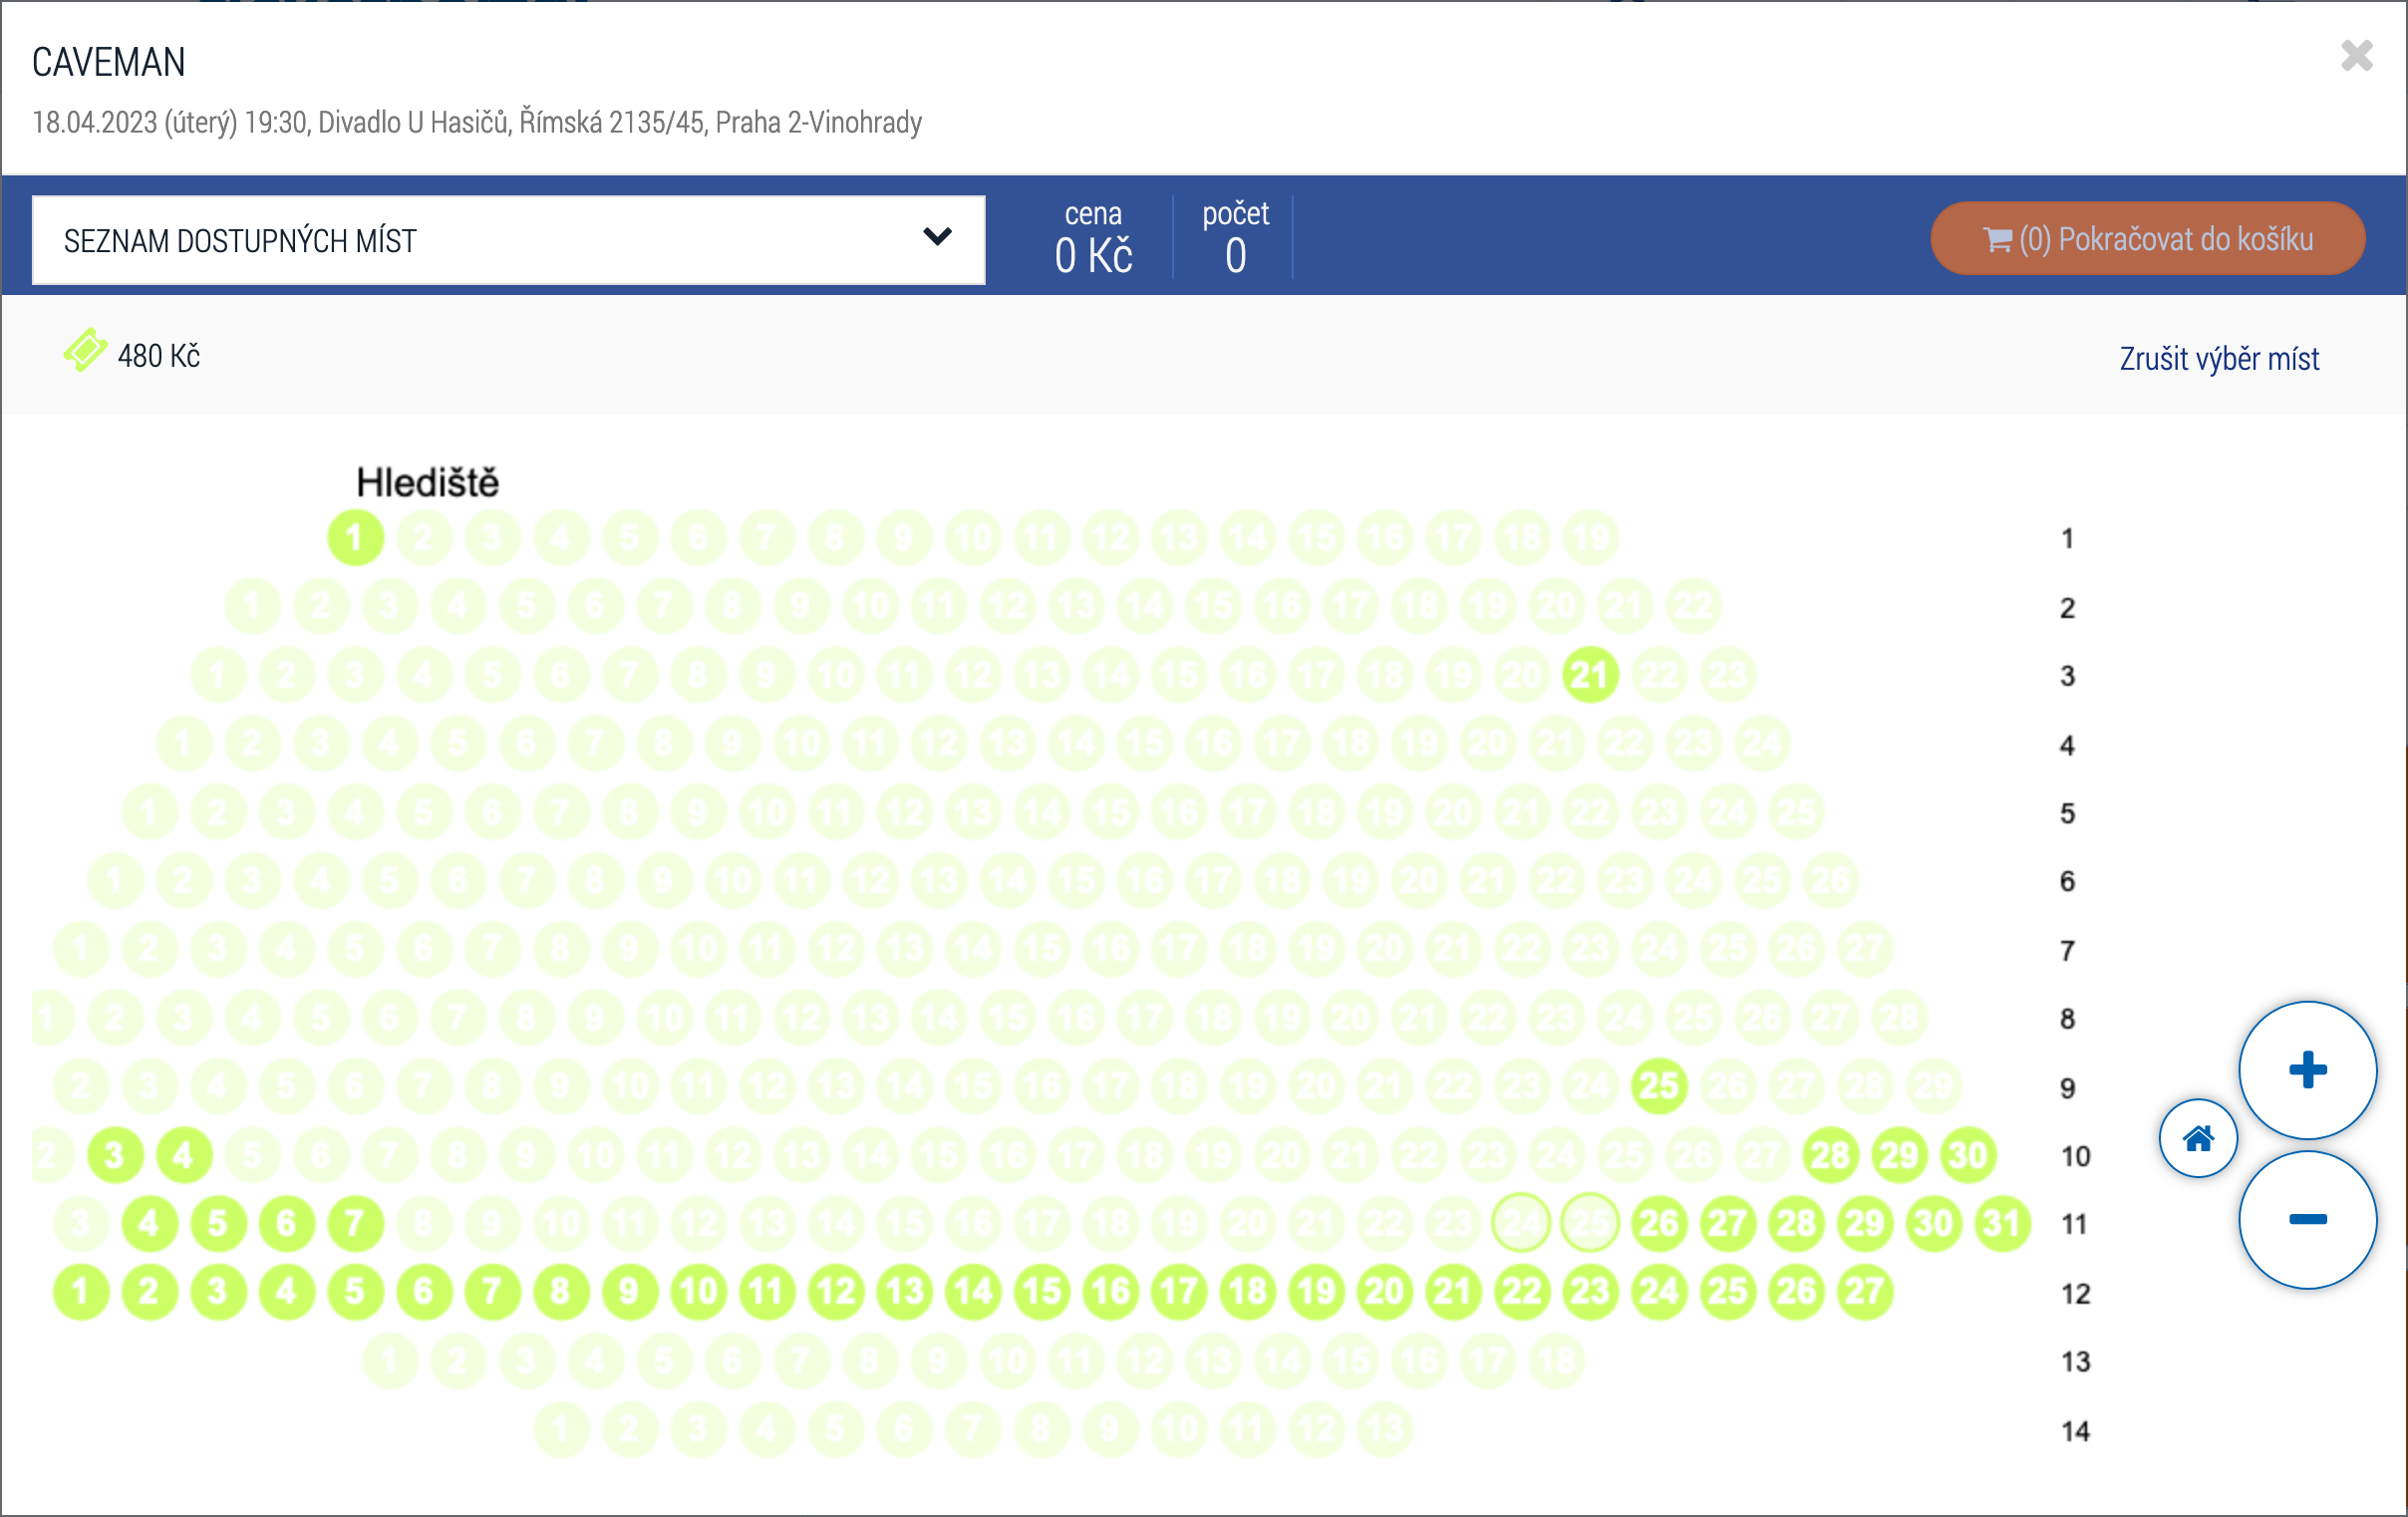
\includegraphics[width=\linewidth]{\FIGDIR/ticketportal-divadlo-u-hasicu}
    \centering
    \caption{Plánek sedaček v síti TICKETPORTAL}
    \label{fig:venue-map-visualization-layout-and-structure}
\end{figure}

Rozložení a struktura prvků na mapě by měly upřednostňovat uživatelskou přívětivost a snadnou navigaci, aby zákazníci mohli rychle najít a vybrat požadovaná místa.
Aby bylo tohoto dosaženo, měla by vizualizace mapy zahrnovat zřetelné sekce, jasné popisky a intuitivní uspořádání míst k sezení či případně i místa vymezená pro stání.

Nejdůležitější prvky, které by mapa měla obsahovat jsou:
\begin{enumerate}
    \item Místa k sezení - zvýrazněná místa k sezení, která jsou k dispozici pro výběr.
    \item Místa pro stání - místa, která jsou určena pro stání, mají větší kapacitu než místa k sezení a jsou také k dispozici pro výběr.
    \item Sektory - rozdělení větších plánku se sedačkami do jednotlivých sektorů seskupujích místa k sezení či stání.
    \item Hlediště - místo, kam budou hledět návštěvníci, důležité pro výběr místa s dobrým výhledem.
    \item Popisky - popisky pro zvýraznění významných míst, jako třeba řady nebo názvy sekcí.
    \item Značky pro zvýraznění dalších objektů - méně důležité, přesto informativní prvky na mapě jako třeba WC, bar, kavárna nebo zábradlí či sloupy.
\end{enumerate}

Tyto prvky by měli být jasně vizuálně definované a na mapě přehledně rozložené.
Záleží převážně o správnou definici a nakreslení prvků na mapě, což je úzce spojeno s administrací mapy a jejího nastavení.
Tu totiž musí někdo prvně vydefinovat a uložit do nějakého datového formátu.
Data si v tomto formátu poté vyžádá aplikace a na jejich základě mapu vykreslí uživateli v prohlížeči.
Touto problematikou se následně více zabývá sekce~\ref{sec:implementace-mapa} v implementační části práce.

%%% Podsekce - Barevné kódování
%%%%% Wording: ⏳
%%%%% Styling: ⏳
%%%%% References: ⏳
%%% --------------------------------------------------------------
\subsection{Barevné kódování}
\label{subsec:specifikace-interaktivni-mapa-barevne-kody}
Barevné kódování je dalším zásadním aspektem vizuálního zobrazení mapy místa konání, protože pomáhá uživatelům rychle identifikovat například kategorie míst, dostupnost a cenové úrovně sedadel.
Díky použití odlišných barev pro různé typy sedadel se zákazník v mapě může snadněji a rychleji orientovat.

Obrázek~\ref{fig:goout-color-codes} zobrazuje plánek míst sezení služby GoOut, který barevně odlišuje různé kategorie míst, dostupnost a cenové úrovně.

\begin{figure}[H]
    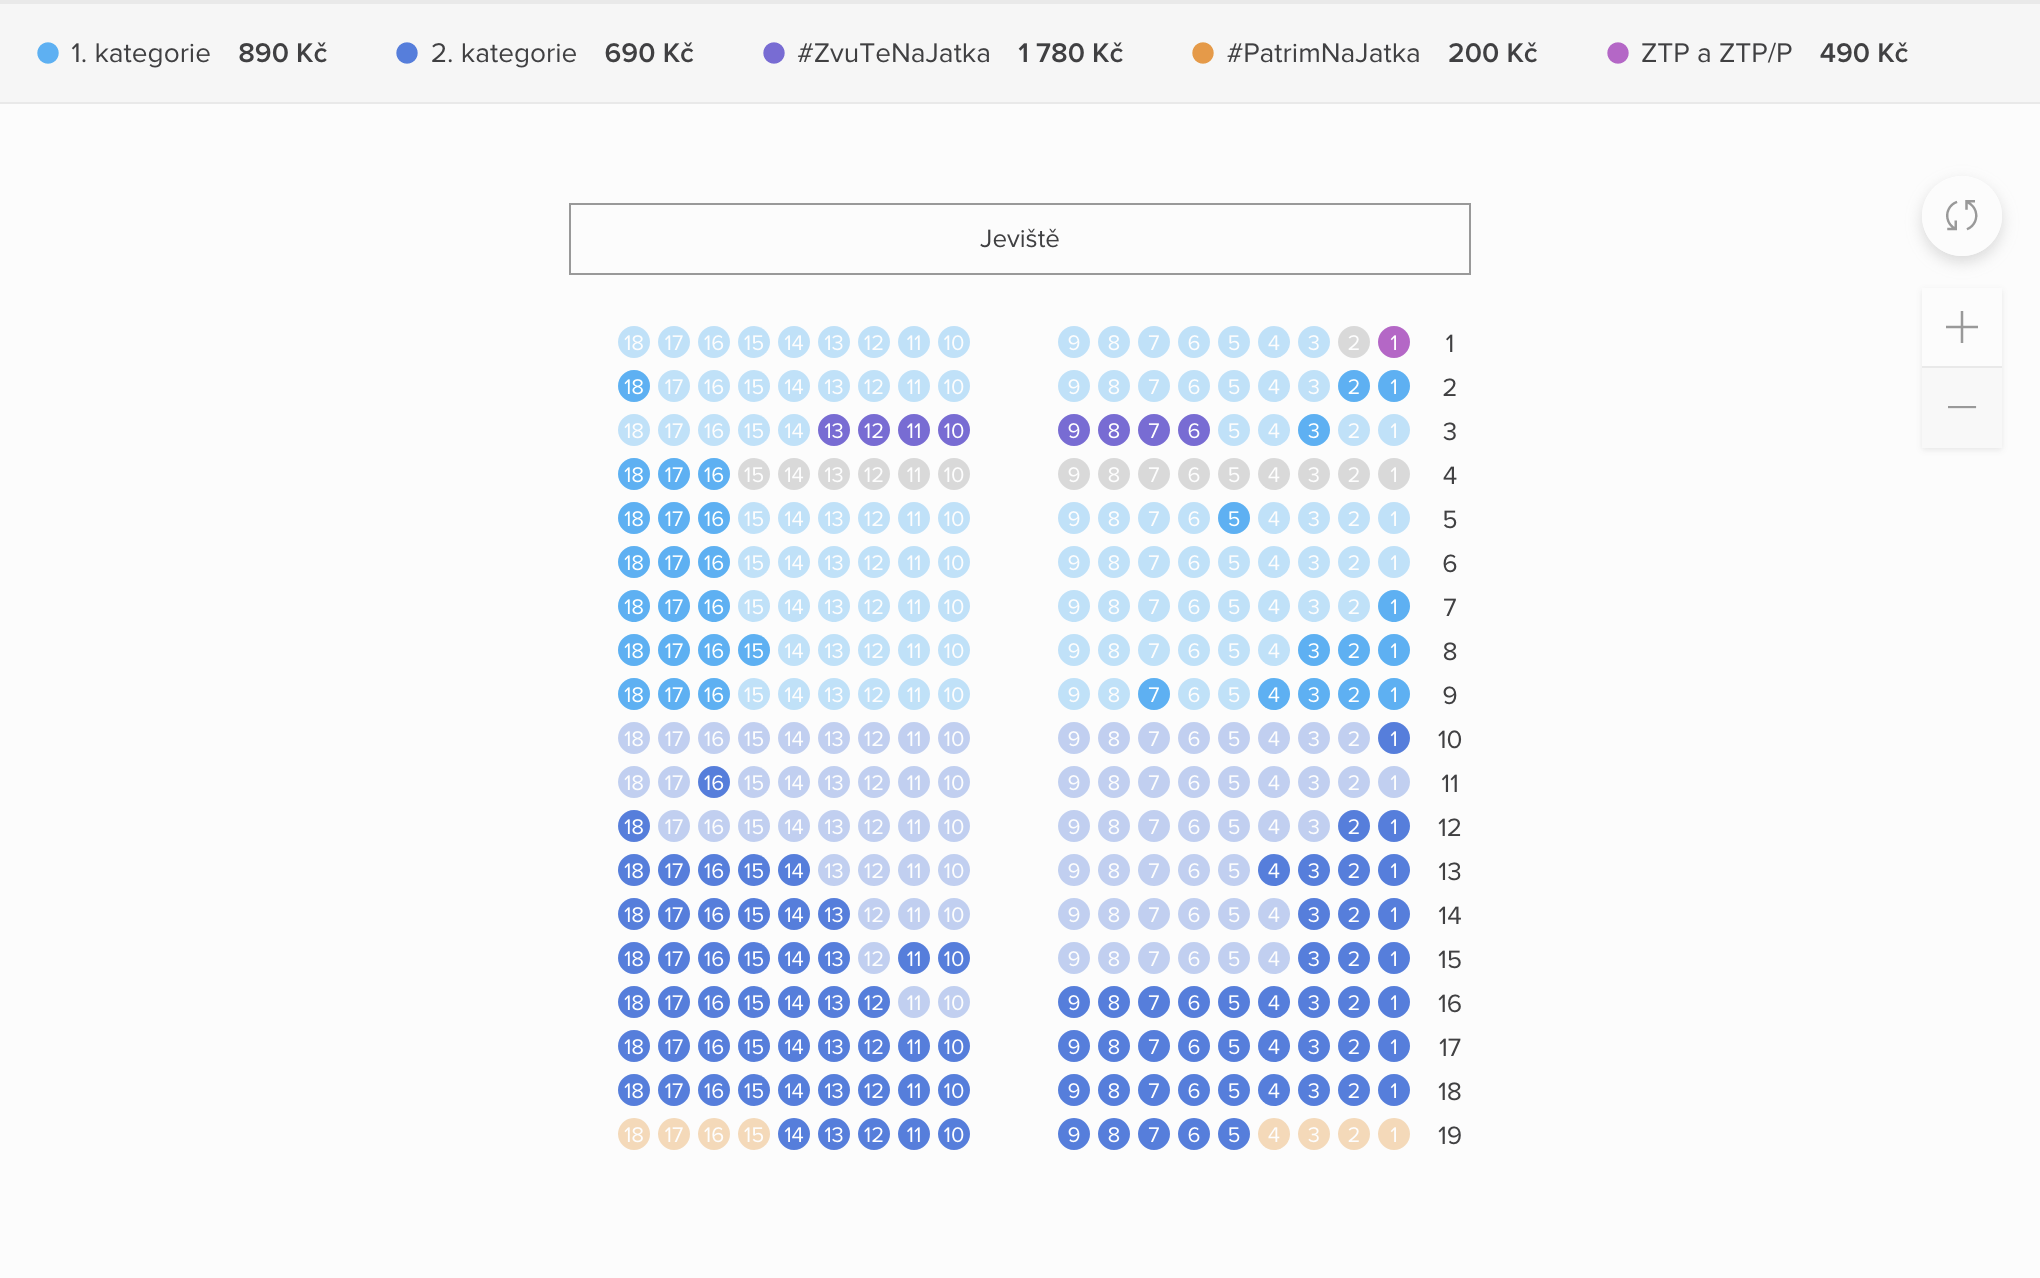
\includegraphics[width=\linewidth]{\FIGDIR/goout-color-codes}
    \centering
    \caption{Mapa barevně odlišených sedadel GoOut}
    \label{fig:goout-color-codes}
\end{figure}

Efektivní implementace barevného kódování vyžaduje použití snadno rozlišitelných barev, které vyhovují zákazníkům s různými zrakovými schopnostmi.
Zvolené barevné schéma by mělo zlepšit přehlednost a zvýšit uživatelský komfort tím, že zjednoduší proces výběru sedadel.
Pro zachování jednotného a přehledného zobrazení je výhodné předem definovat paletu barev, které budou moci být později použity pro různé prvky na mapě.
Užitím palety barev lze také jednodušeji udržet jednotnout vizuální identitu mapy a lze také předcházet zobrazenímu nekontrastních barevných kombinací, například textu na barevném podkladu.

%%% Podsekce - Ovládání mapy
%%%%% Wording: ⏳
%%%%% Styling: ⏳
%%%%% References: ⏳
%%% --------------------------------------------------------------
\subsection{Ovládání mapy}
\label{subsec:specifikace-interaktivni-mapa-ovladani}
Ovládání zobrazení mapy je důležitou částí implementace, jelikož dodává větší interaktivnost tím, že umožňuje například pohyb kamery mapy po ose \em{x} a \em{y}, rotaci či přiblížení a oddálení.
Tyto funkce zákazníkovi umožňují podrobněji prozkoumat celou mapu místa a zároveň zobrazit více informací na jednom zobrazení.
Díky těmto funkcím získá zákazník také lepší přehled o celkovém rozpoložení míst v areálu.
Takovéto funkce jsou esenciální u zobrazení map větších areálů jako jsou například arény či stadiony.
Tyto mapy jsou totiž většinou ještě rozděleny do sektorů, které seskupují místa k sezení či stání.
Použitím funkce přiblížení a oddeálení lze také zobrazit různé úrovně detailu prvků na mapě v závislosti právě na hodnotě přiblížení.

Tento přístup například využívá síť \foreign{Ticketmaster}, který je možno vidět na obrázku~\ref{fig:ticketmaster-o2-zoom}, kde je demonstrována mapa sedadel s funkcí přiblížení a posunu a také s rozdělením na sektory.
Při oddálení mohou uživatelé zobrazit celkové rozložení místa konání rozdělené do sektorů.
Po přiblížení se zobrazí podrobnější zobrazení jednotlivých míst ve vybraném sektoru, což uživatelům umožňuje podrobně prozkoumat konkrétní oblasti areálu a vybrat požadované místo.

\begin{figure}[H]
    \centering
    \begin{subfigure}{0.45\textwidth}
        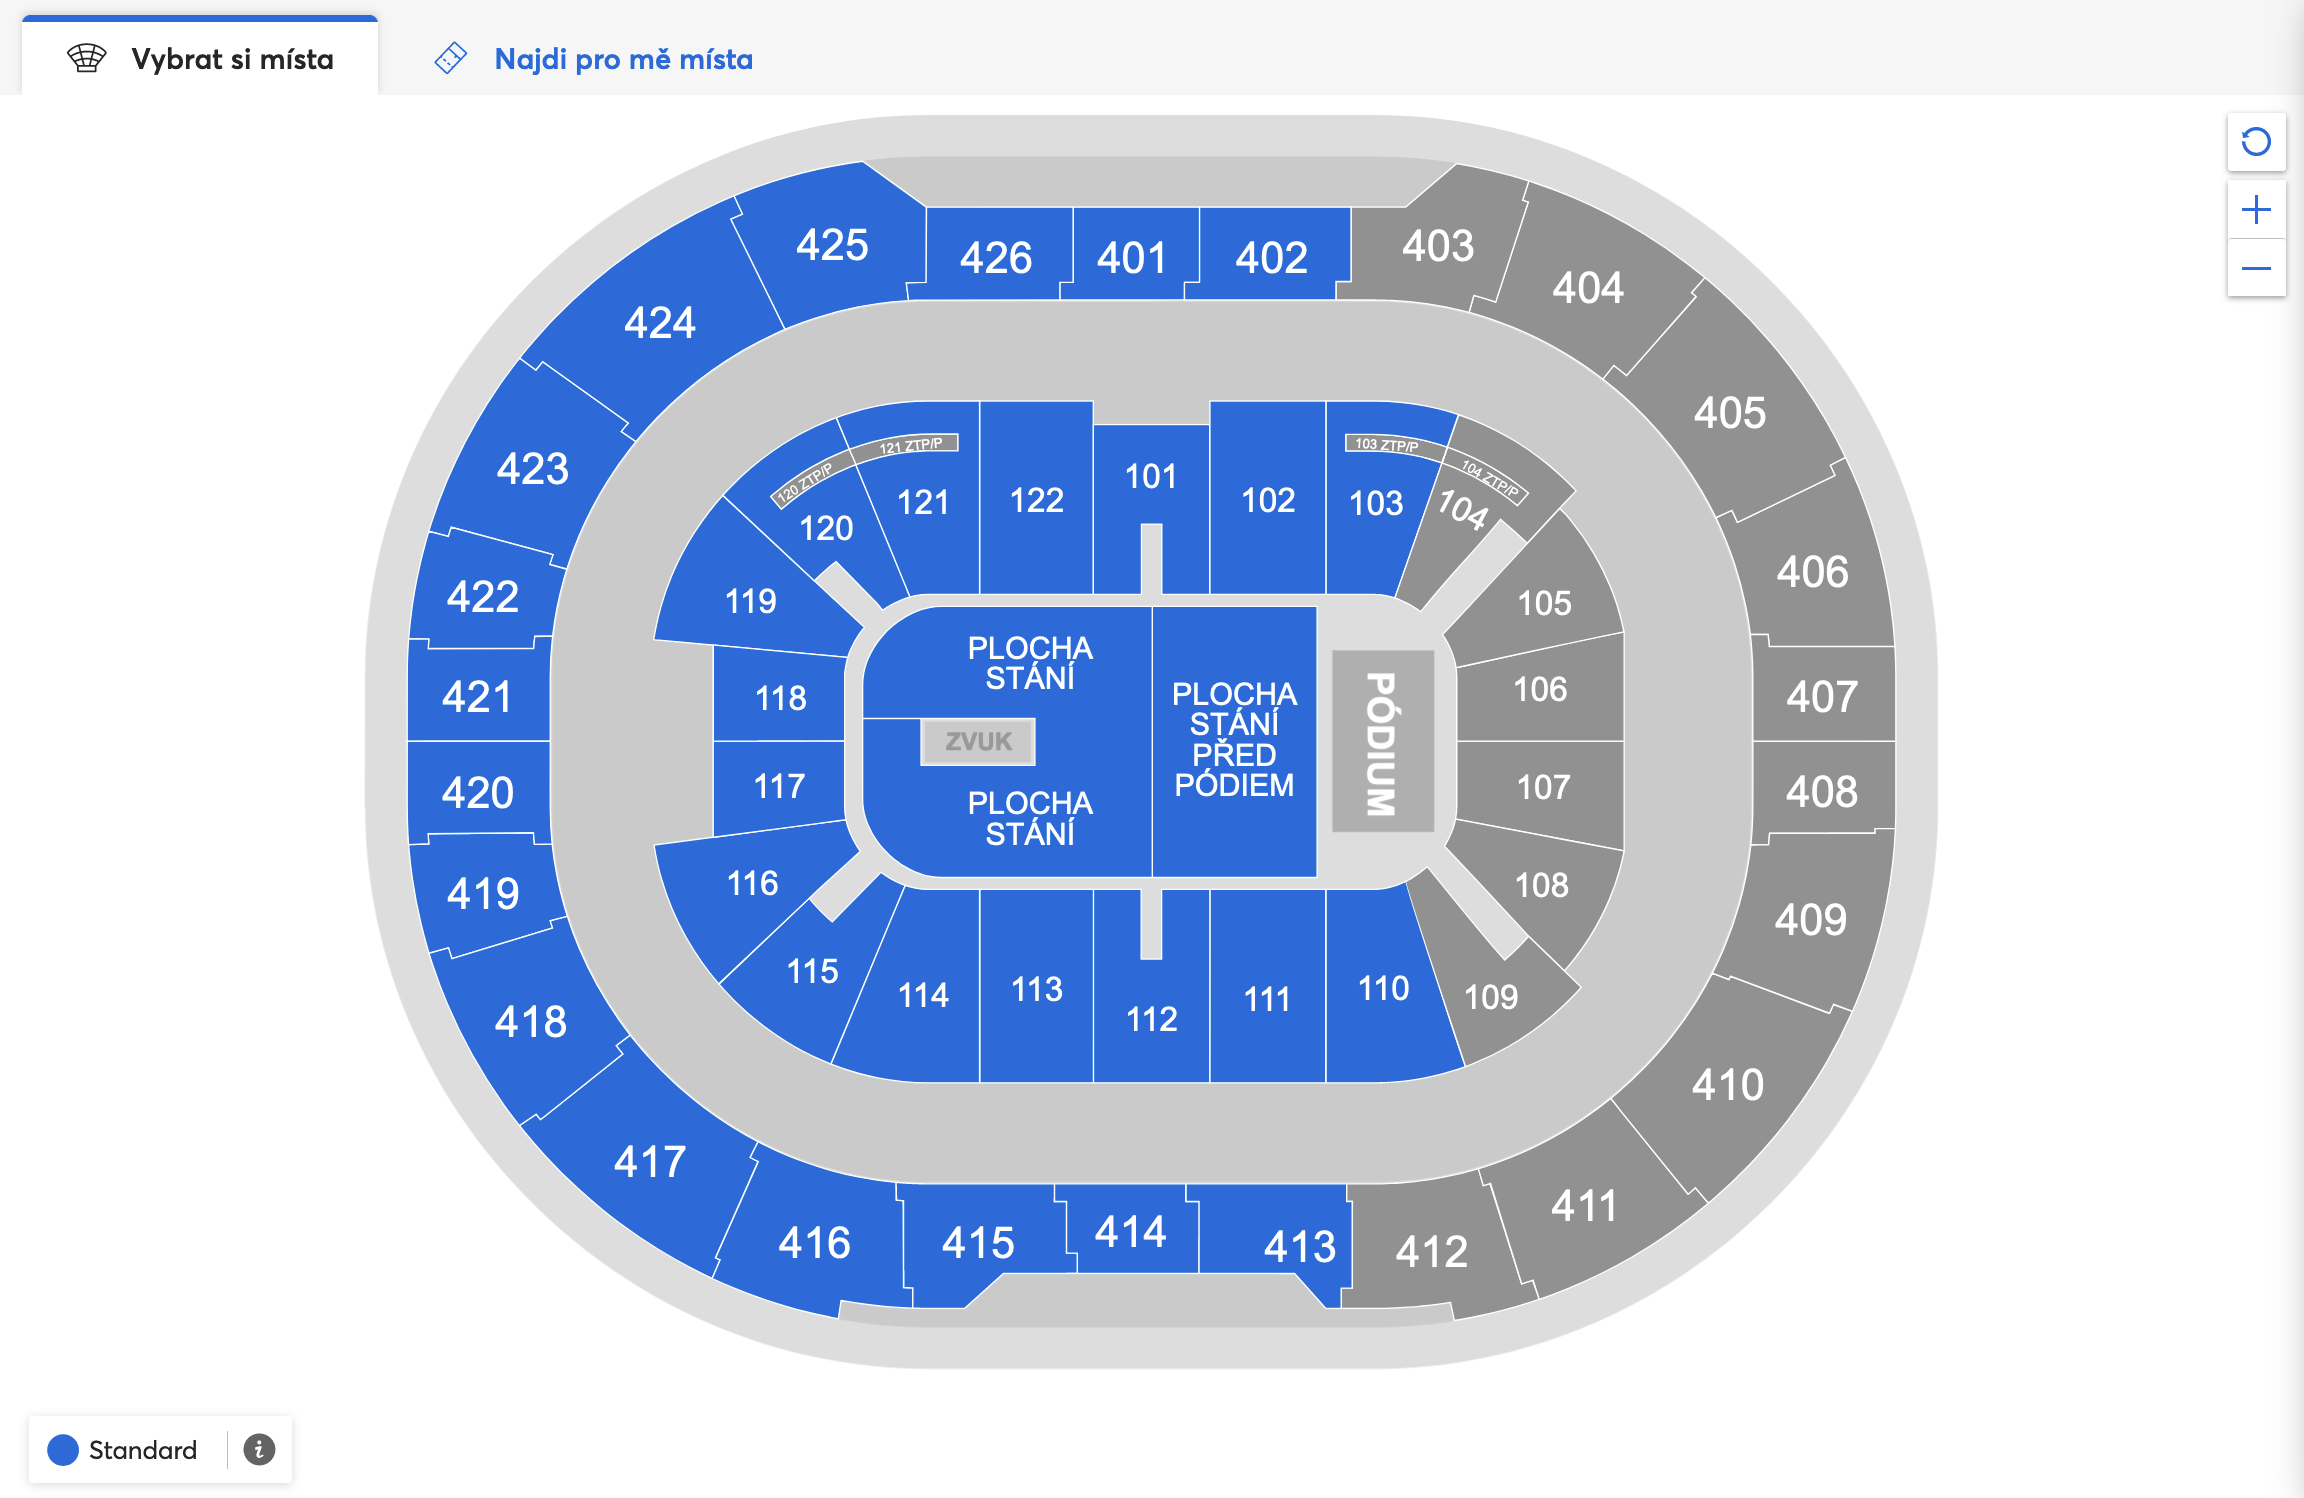
\includegraphics[width=\textwidth]{\FIGDIR/ticketmaster-o2-zoom-out}
        \caption{Oddálený pohled}
        \label{fig:ticketmaster-o2-zoom-in}
    \end{subfigure}
    \hfill
    \begin{subfigure}{0.45\textwidth}
        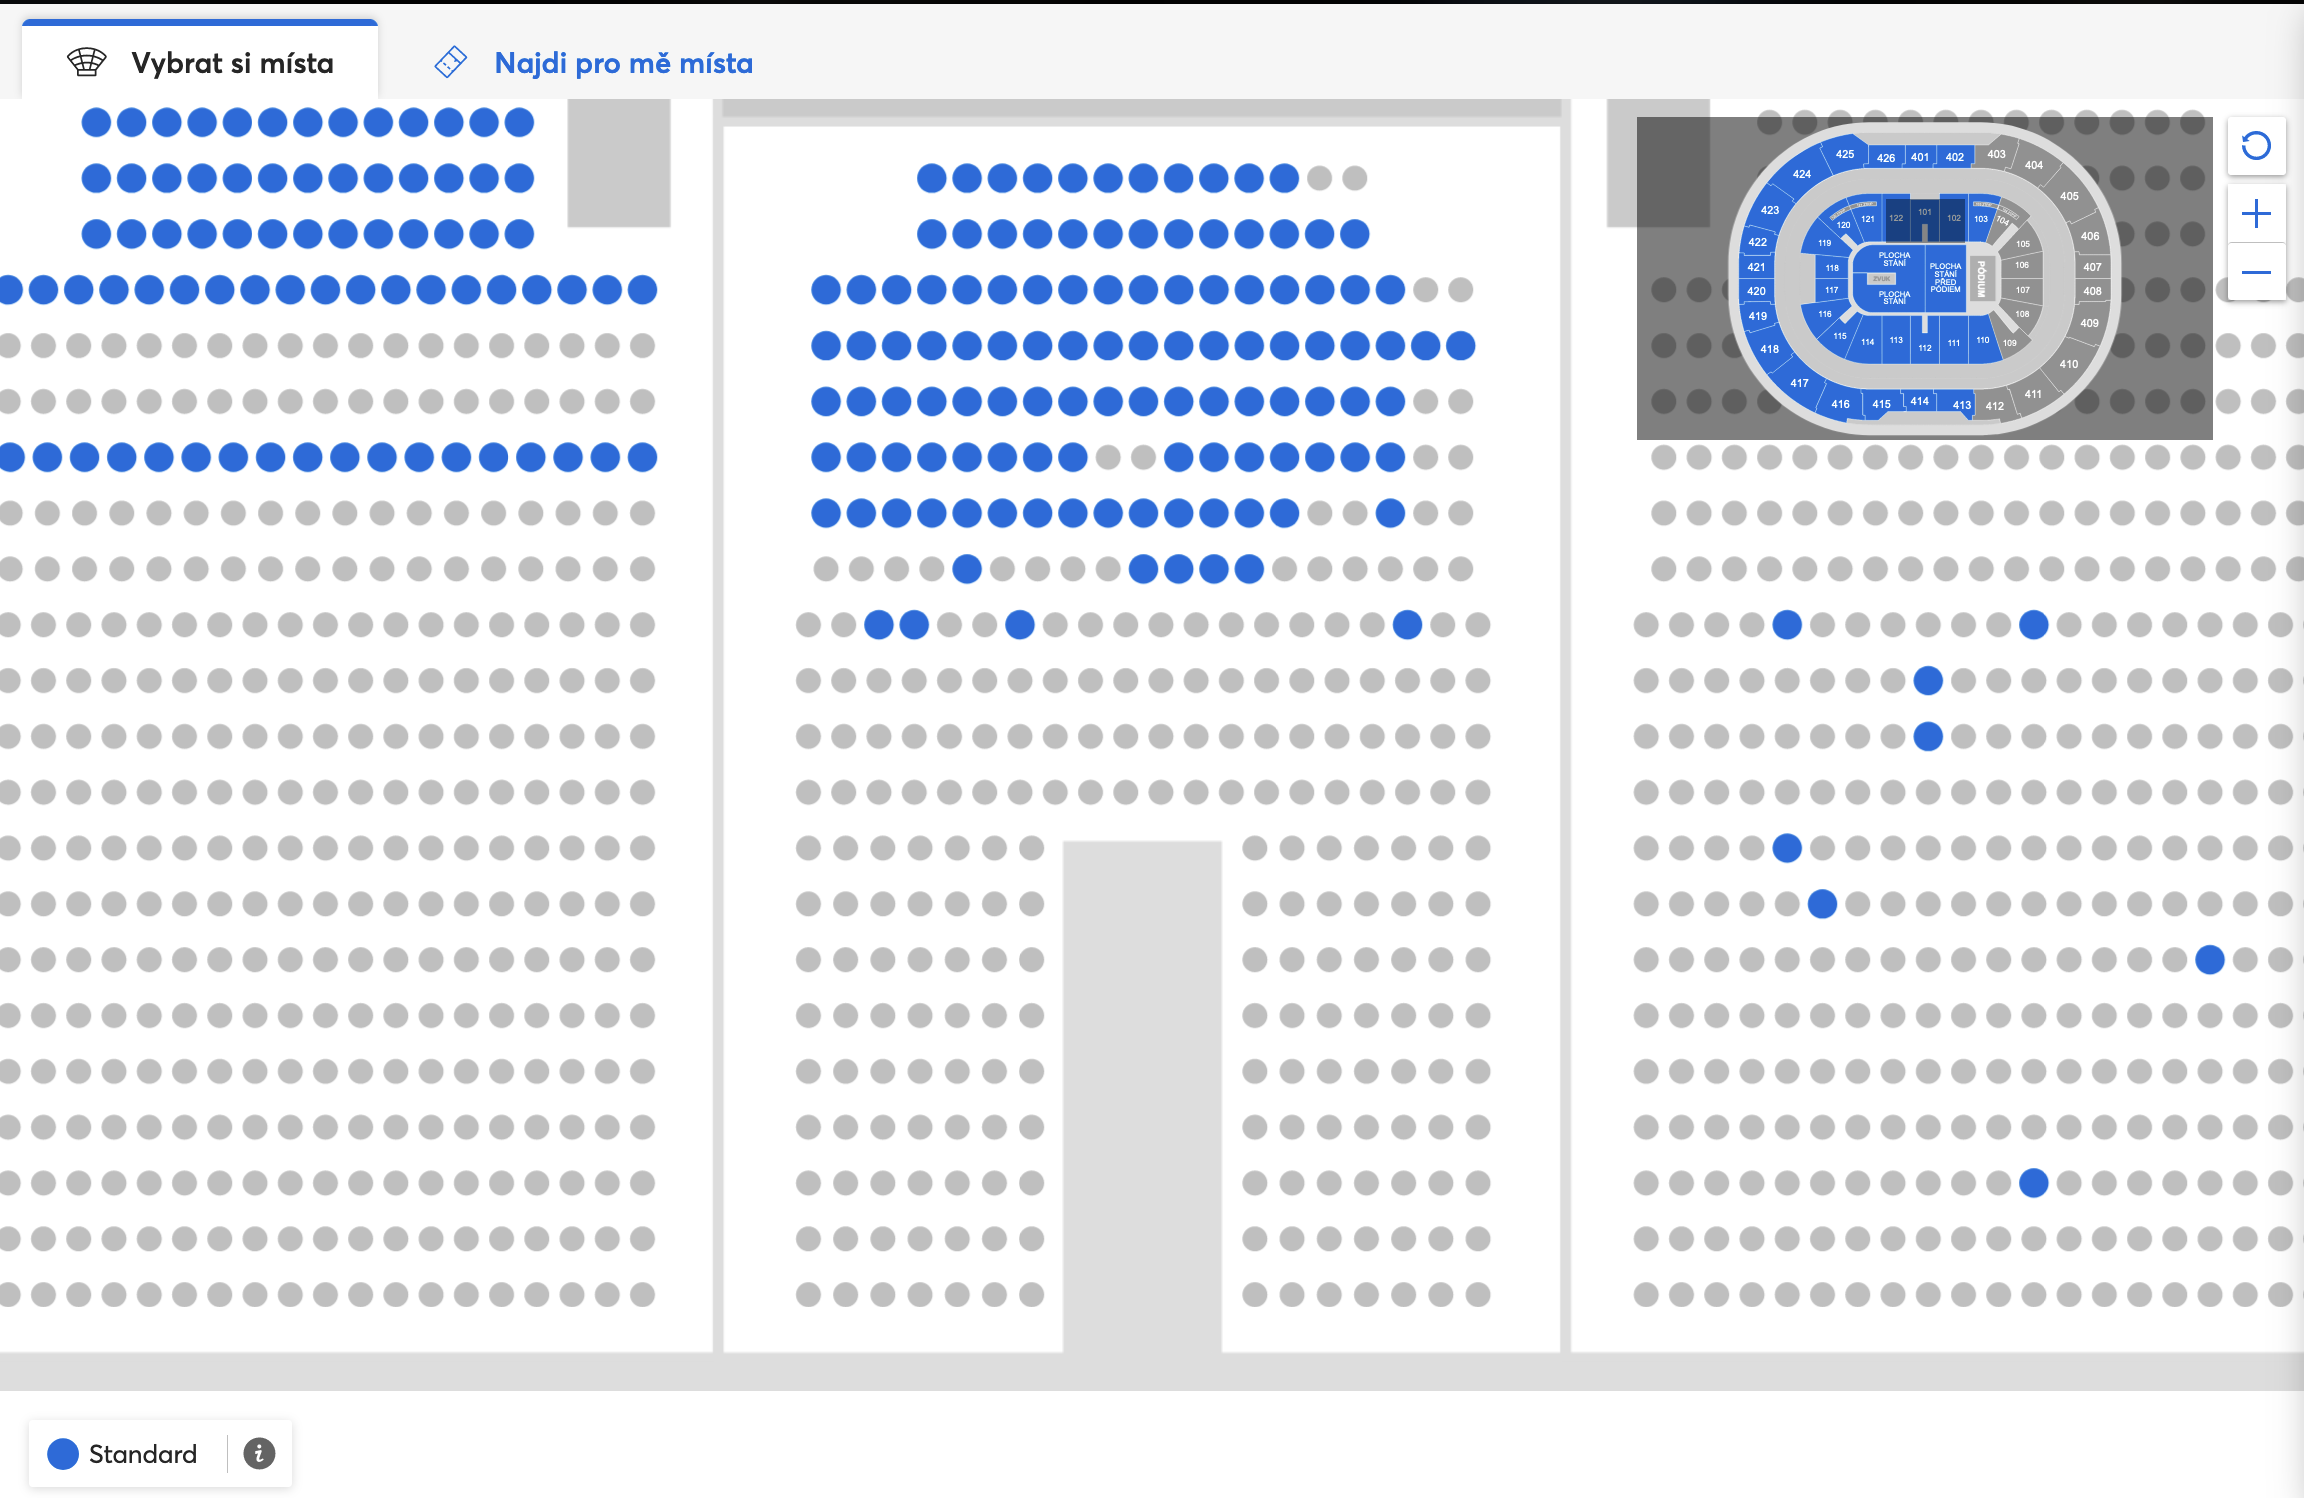
\includegraphics[width=\textwidth]{\FIGDIR/ticketmaster-o2-zoom-in}
        \caption{Přiblížený pohled}
        \label{fig:ticketmaster-o2-zoom-out}
    \end{subfigure}

    \caption{Různé pohledy mapy v síti Ticketmaster.}
    \label{fig:ticketmaster-o2-zoom}
\end{figure}

Při implementaci těchto funkčností je důležité myslet na přístupnost z pohledu koncových zařízení.
Například pro nedotyková zařízení tyto funkčnosti zajišťují ukazovací zařízení jako počítačové myši.
Na dotykových zařízeních jsou tyto funkčnosti docíleny pomocí dotykových gest \foreign{pinch} a \foreign{zoom} pro simulaci přiblížení a oddálení, gesta \foreign{rotate} pro rotaci a gesta \foreign{pan} pro pohyb na osách mapy.
Je tedy třeba zajistit podporu pro dotyková i nedotyková zařízení.
Často se k mapám zobrazuje i lišta s nástroji, které tyto funkčnosti ovládají.
V těchto lištách je také vhodné umístit tlačítko na vrácení zobrazení mapy do výchozího zobrazení.

%%% Podsekce - Stav a informace o sedadlech
%%%%% Wording: ⏳
%%%%% Styling: ⏳
%%%%% References: ⏳
%%% --------------------------------------------------------------
\subsection{Stav a informace o sedadlech}
\label{subsec:specifikace-interaktivni-mapa-stav-a-informace-o-sedadlech}
Sedadla a ostatní místa k výběru o sobě nesou informace, které na mapě nemusejí být zřejmá a které zákazníkovi usnadňují výběr místa.
Tyto informace mohou být pro zákazníka zásadní, jelikož poskytují podrobnosti, jako je dostupnost, cena, přístupnost či další jiné popisy.
Díky těmto informacím se zákazník může lépe rozhodnout a vybrat si sedadlo, které nejlépe vyhovuje jeho preferncím a požadavkům.

Obrázek~\ref{fig:ticketmaster-o2-seat-info} zobrazuje mapu sedadel se stavem a informacemi o zvoleném sedadlu.
Uživatelé si mohou zobrazit  dostupnost, cenu a další důležité údaje o jednotlivých místech, což jim usnadňuje výběr preferovaných míst k sezení.

\begin{figure}[H]
    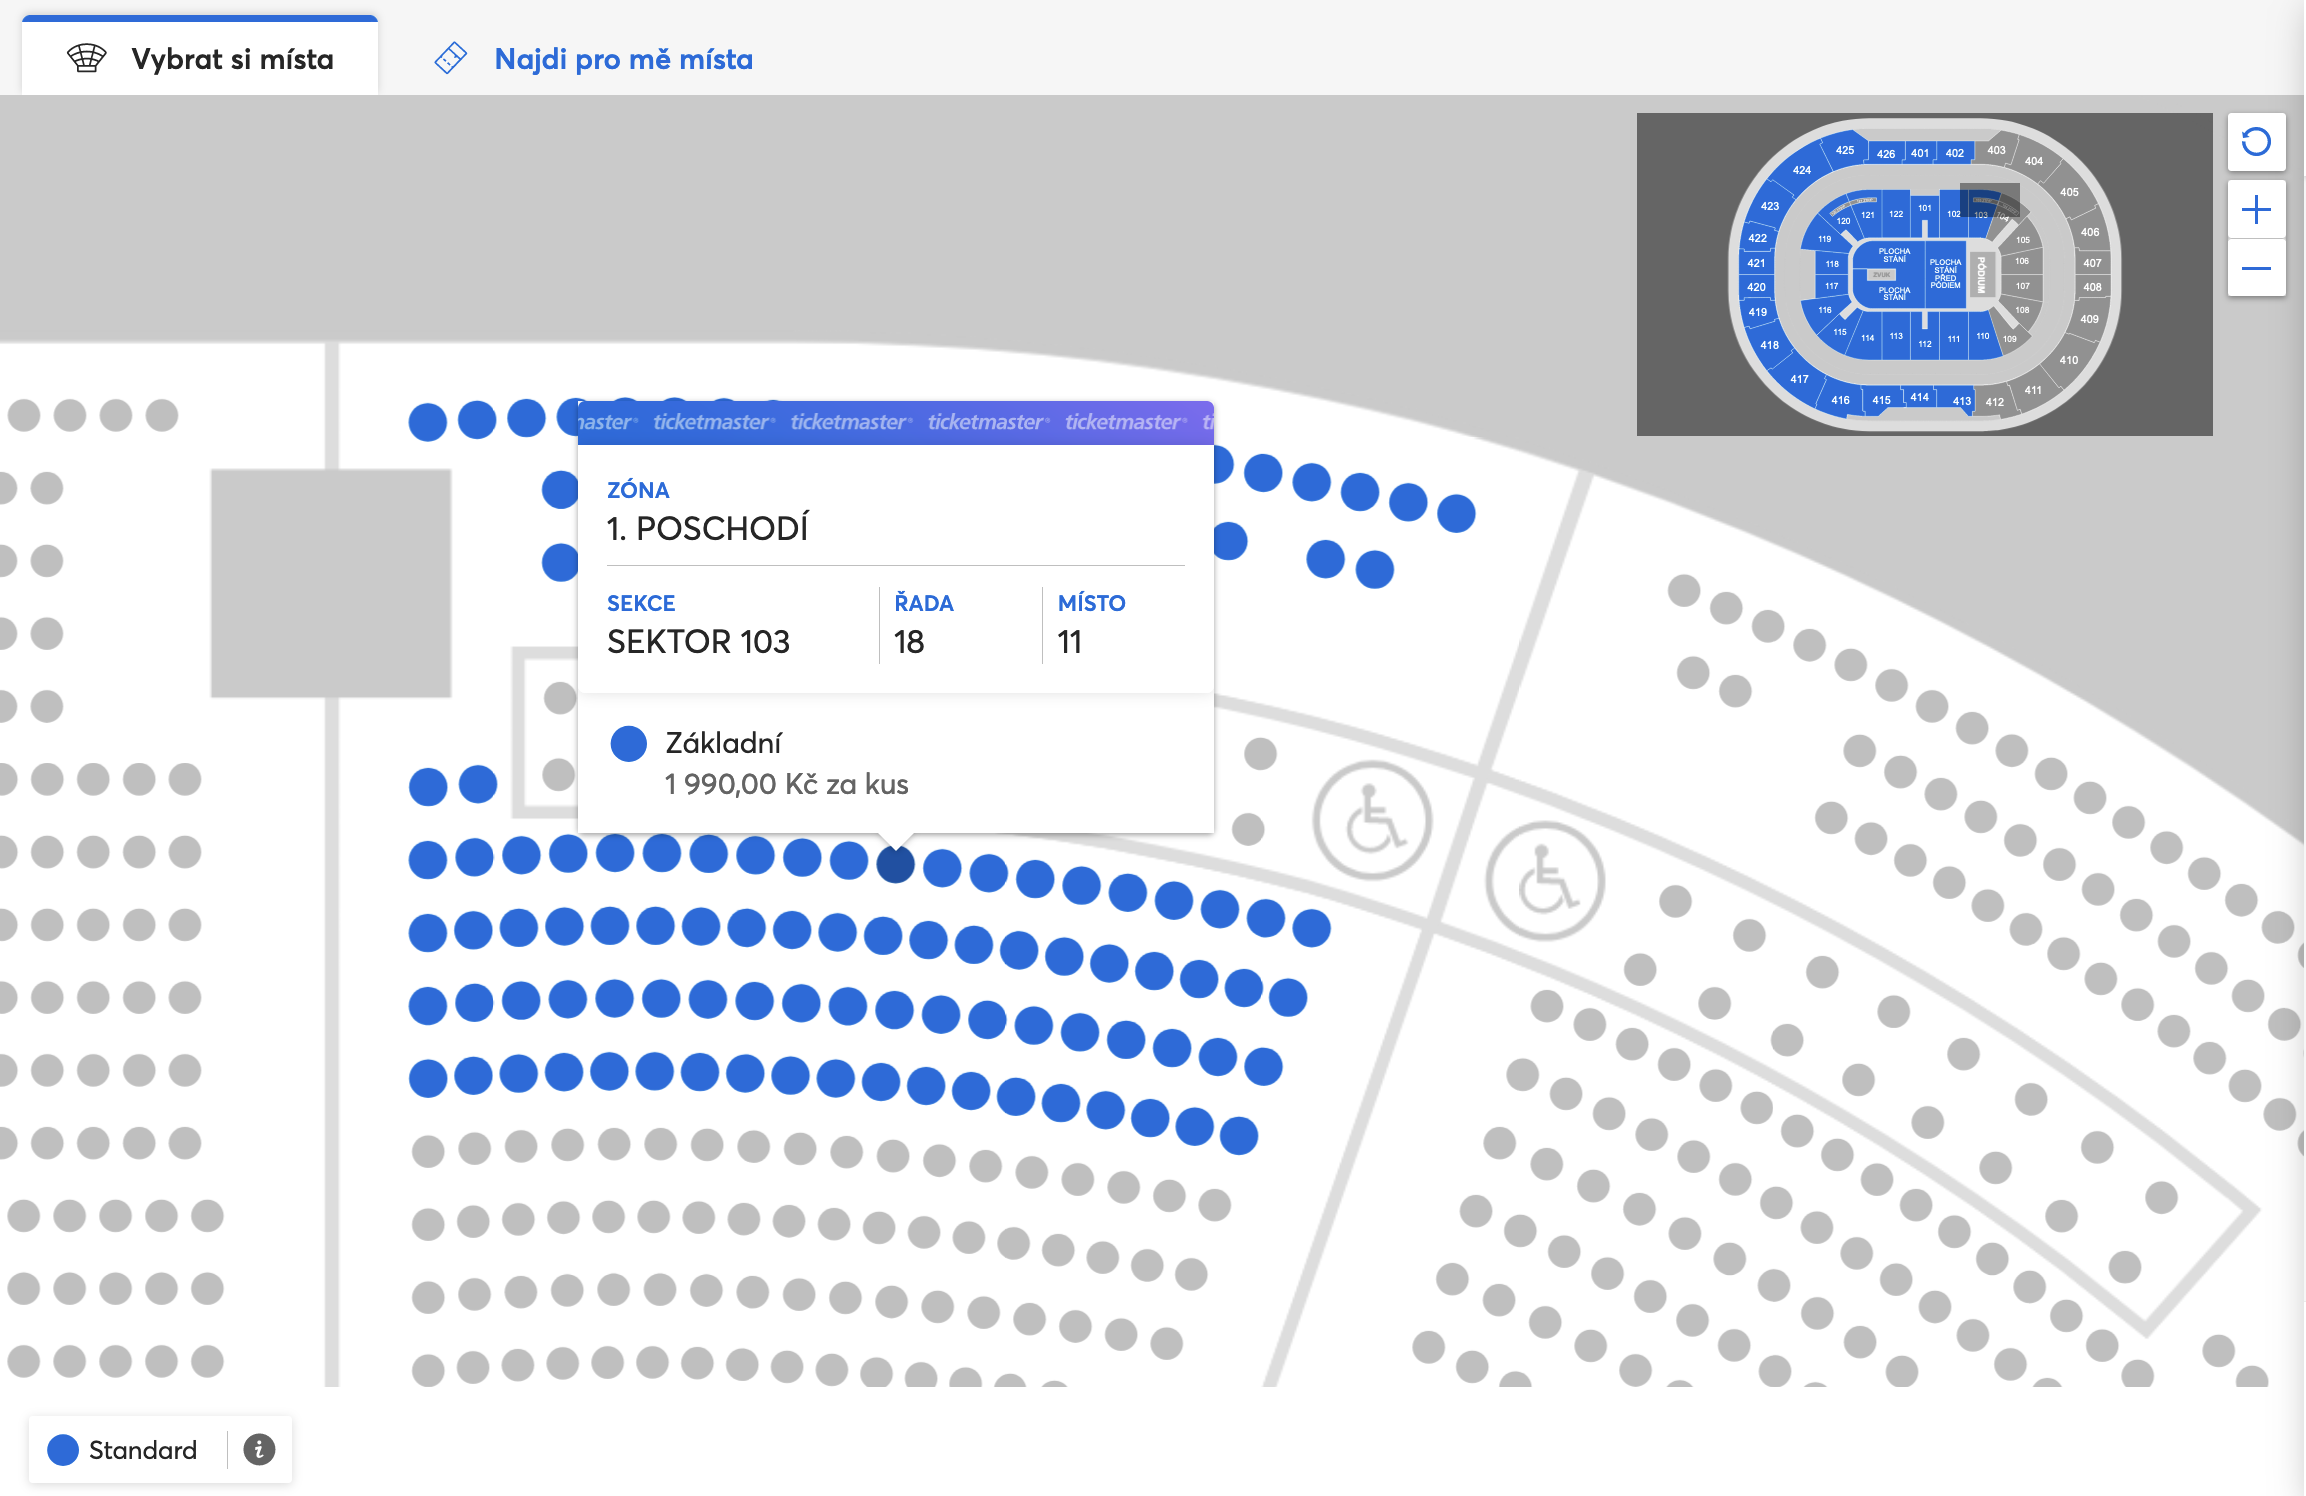
\includegraphics[width=\linewidth]{\FIGDIR/ticketmaster-o2-seat-info}
    \centering
    \caption{Informace o sedadle na mapě v síti Ticketmaster.}
    \label{fig:ticketmaster-o2-seat-info}
\end{figure}

Aby bylo možné efektivně implementovat informace o stavu sedadel, měla by být mapa míst jasná a srozumitelná a všechny důležité údaje by měly být snadno dostupné.
Jedním z běžných přístupů je použití vyskakovacích oken typu \foreign{popover} s informacemi, které se zobrazí  například po najetí myší.
Tato metoda však nemusí být vhodná pro mobilní a dotyková zařízení, kde takováto podobná gesta nefungují či fungují hodně omezeně.
Pro řešení tohoto problému lze použít alternativní přístup, a to například zobrazení informací o sedadle ve vyjíždějící spodní či boční liště po označení na sedadla.
Tím je zajištěno, že stav sedadla a informace o něm jsou přístupné uživatelům na všech zařízeních.

Toto okno či lišta by měla obsahovat ty nejdůležitější informace o zvoleném místě, jako:
\begin{enumerate}
    \item Řada a místo - číselné či alfanumerické označení řady a místa sedačky.
    \item Sektor - pokud je mapa rozdělena do sektorů, tak sektor, ve kterém se sedačka nachází.
    \item Cenu - cenu vstupenky odpovídající dané sedačce.
    \item Barevné označení - barevné označení sedačky, například dle její cenové kategorie.
    \item Stav sedačky - stav, ve kterém se sedačka vůči zákazníkovi nachází (obsazená, zvolená, nedostupná, \ldots).
    \item Další atributy - další informativní atributy, jako například informace o zhoršených podmínkách viditelnosti nebo vyhrazení místa pro osoby s postižením.
\end{enumerate}


%%% Podsekce - Data a jejich dostupnost
%%%%% Wording: ⏳
%%%%% Styling: ⏳
%%%%% References: ⏳
%%% --------------------------------------------------------------
\subsection{Data a jejich dostupnost}
\label{subsec:specifikace-interaktivni-mapa-data-a-dostupnost}
Pro zobrazení a fungování aplikace je nezbytné mapu a celý její stav zkonstruovat pomocí reálných a aktualizovaných dat dostupných z backendového systému pomocí aplikačního rozhraní, označovaného jako \foreign{API}.
Tato data obsahují informace o vstupenkách a sedačkách jako například dostupnost, cena, umístění a další ostatní relevantní informace.
Struktura těchto dat by měla být jasně definovaná a dostupná ve formátu vyhovujícímu užití aplikace.

Areály s velkým množství sedaček mohou být problematické a to převážně z pohledu objemu přenášených dat mezi klientem a API\@.
Je důležité myslet na implementaci inteligentního datového přenosu, který zajistí komunikaci a přenos pouze nezbytných dat.
Díky menšímu objemu přenášených dat se pak zdá aplikace rychlejší a responzivnější.

Dalším aspektem práce s daty v takovéto aplikaci je aktualizace dat o dostupnosti.
Tato funkčnost zajišťuje zákazníkovi zobrazení aktuálních informací o sedačkách či vstupenkách a snižuje tak například riziko konfliktu výběru již obsazené sedačky.
Průběžné aktualizace dat lze docílit technologiemi jako například \foreign{WebSockets} nebo částečnými aktualizacemi dotazovanými skrze API\@.
Tyto metody budou později rozebrány v implementační části práce.


%%% Sekce - Nákupní košík
%%%%% Wording: ⏳
%%%%% Styling: ⏳
%%%%% References: ⏳
%%% --------------------------------------------------------------
\section{Nákupní košík}
\label{sec:specifikace-nakupni-kosik}
Velmi důležitou součástí fungování celého systému je efektivní správa a vizualizace nákupního košíku.
Ta například zákazníkovi poskytuje přehledný souhrn položek, které si objednává, a umožňuje mu je případně upravit či odebrat.
Nicméně ale tím nejdůležitejším aspektem nákupního košíku jsou jaká data jsou v něm uchovány a jakým způsobem jsou zpracována.

Tato podkapitola se zabývá popisem hlavním funkčností a požadavků na nákupní košík, které jsou nezbytné pro jeho efektivní fungování v rámci webového řešení s využitím rezervace sedadel.

\begin{figure}[H]
    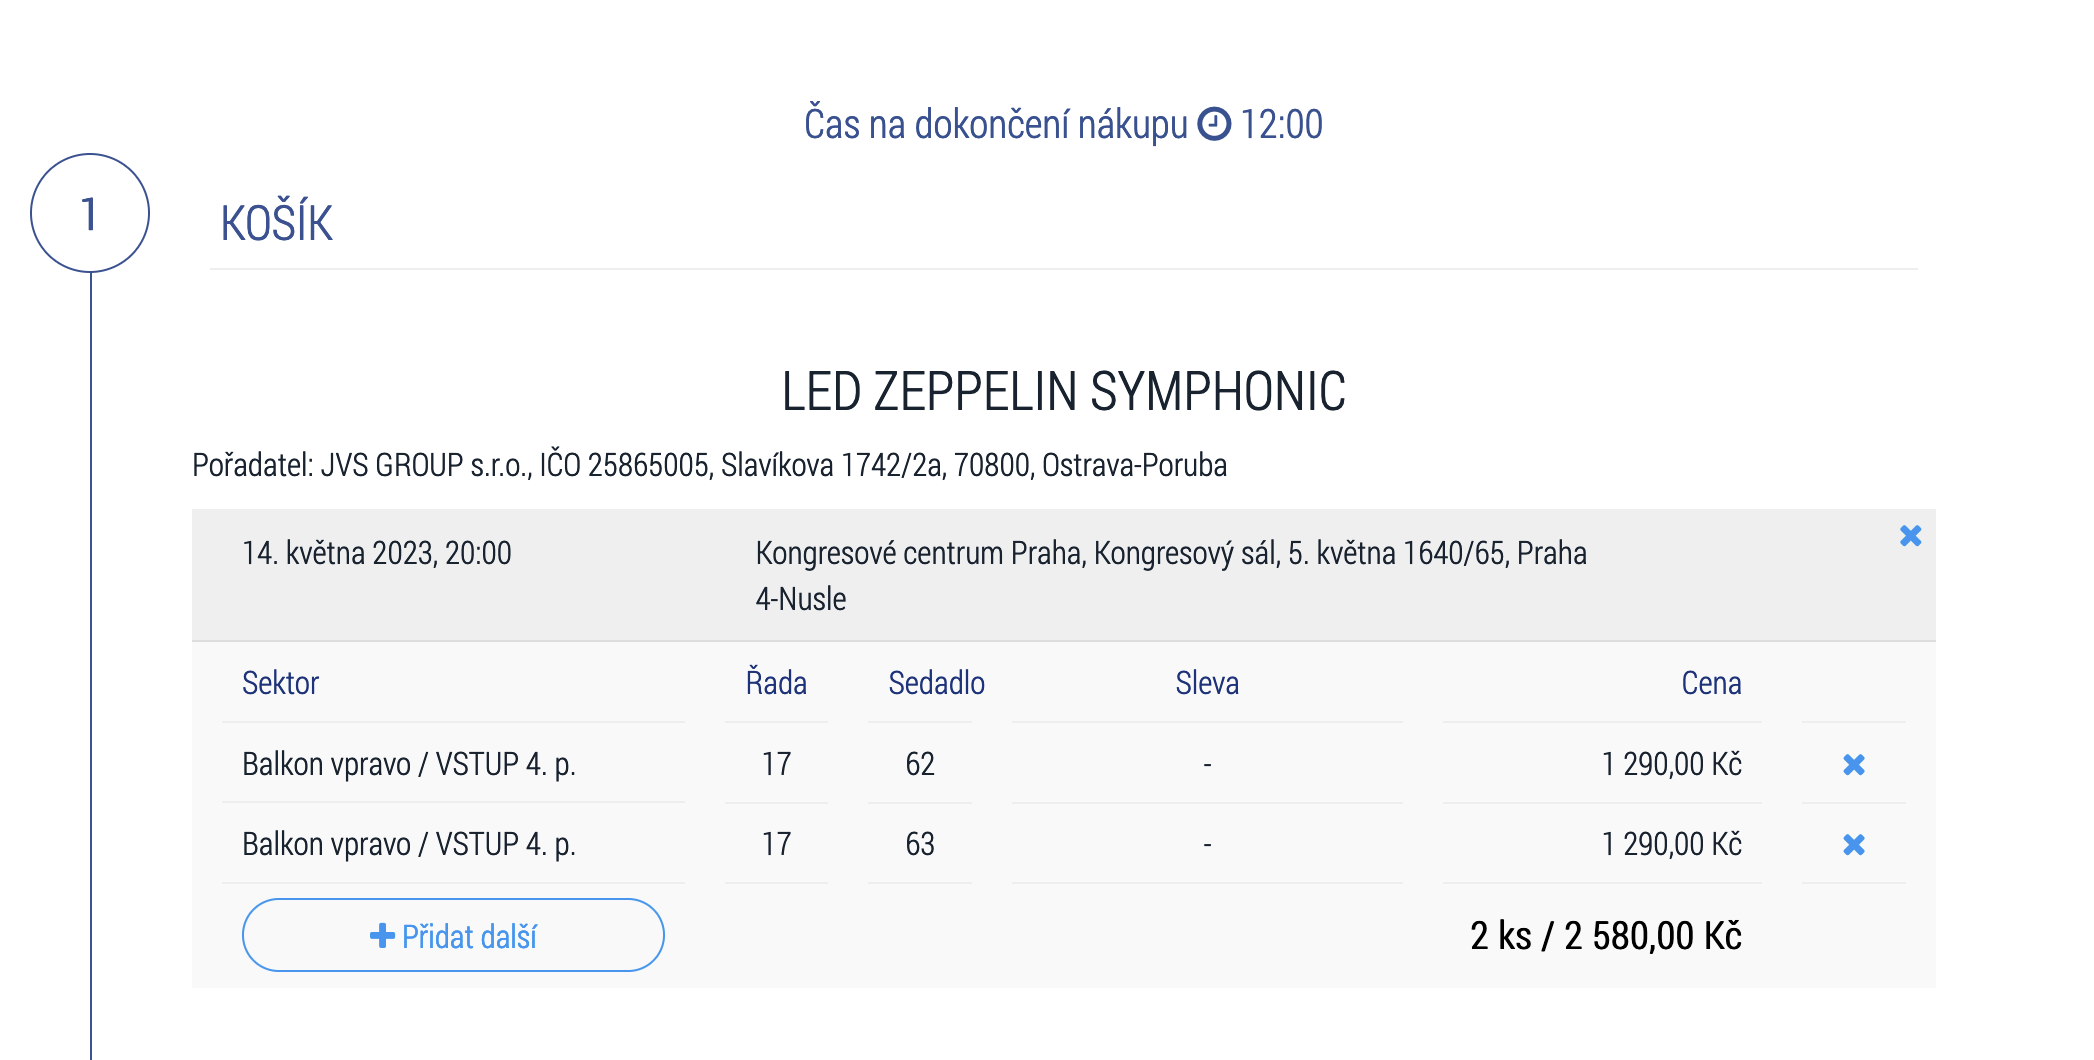
\includegraphics[width=\linewidth]{\FIGDIR/ticketportal-cart}
    \centering
    \caption{Obsah nákupního košíku na portálu Ticketportal.cz}
    \label{fig:ticketportal-cart}
\end{figure}

%%% Podsekce - Správa dat
%%%%% Wording: ⏳
%%%%% Styling: ⏳
%%%%% References: ⏳
%%% --------------------------------------------------------------
\subsection{Správa dat}
\label{subsec:specifikace-nakupni-kosik-sprava}
Nákupní košík by z datové perspektivy měl být implementován jako objekt, který uchovává informace o všech vybraných sedačkách a vstupenkách.
Datová struktura a uchovávaná data uvnitř daného objektu o stavu nákupního košíku by měla být jasně definovaná a dostupná ve formátu vyhovujícímu užití aplikace.
Díky těmto datům by mělo být vždy možné zrekonstruovat stav nákupního košíku a to i v případě, že uživatel opustí stránku nebo zavře prohlížeč.

Touto problematikou se bude primárně zabývat kapitola~\ref{sec:implementace-kosik}, ve které bude podrobně popsána datavá struktura a finální funkčnost nákupního košíku.

%%% Podsekce - Přehled obsahu košíku
%%%%% Wording: ⏳
%%%%% Styling: ⏳
%%%%% References: ⏳
%%% --------------------------------------------------------------
\subsection{Přehled obsahu košíku}
\label{subsec:specifikace-nakupni-kosik-prehled}
Pro zákazníka nákupní košík slouží primárně k přehlednému zobrazení všech vybraných položek, které budou tvořit jeho objednávku.
V případně této webové aplikace se primárně jedná o vstupenky a zarezervované sedačky.

Zákazník by měl být schopen jednoduše zjistit, jaké položky si objednává a jaké mají parametry.
Seznam všech těchto položek posléze tvoří celkový přehled nákupního košíku, který umožňuje zákazníkovi zkontrolovat jeho výběr a provést případné změny před dokončením objednávky.

\begin{figure}[H]
    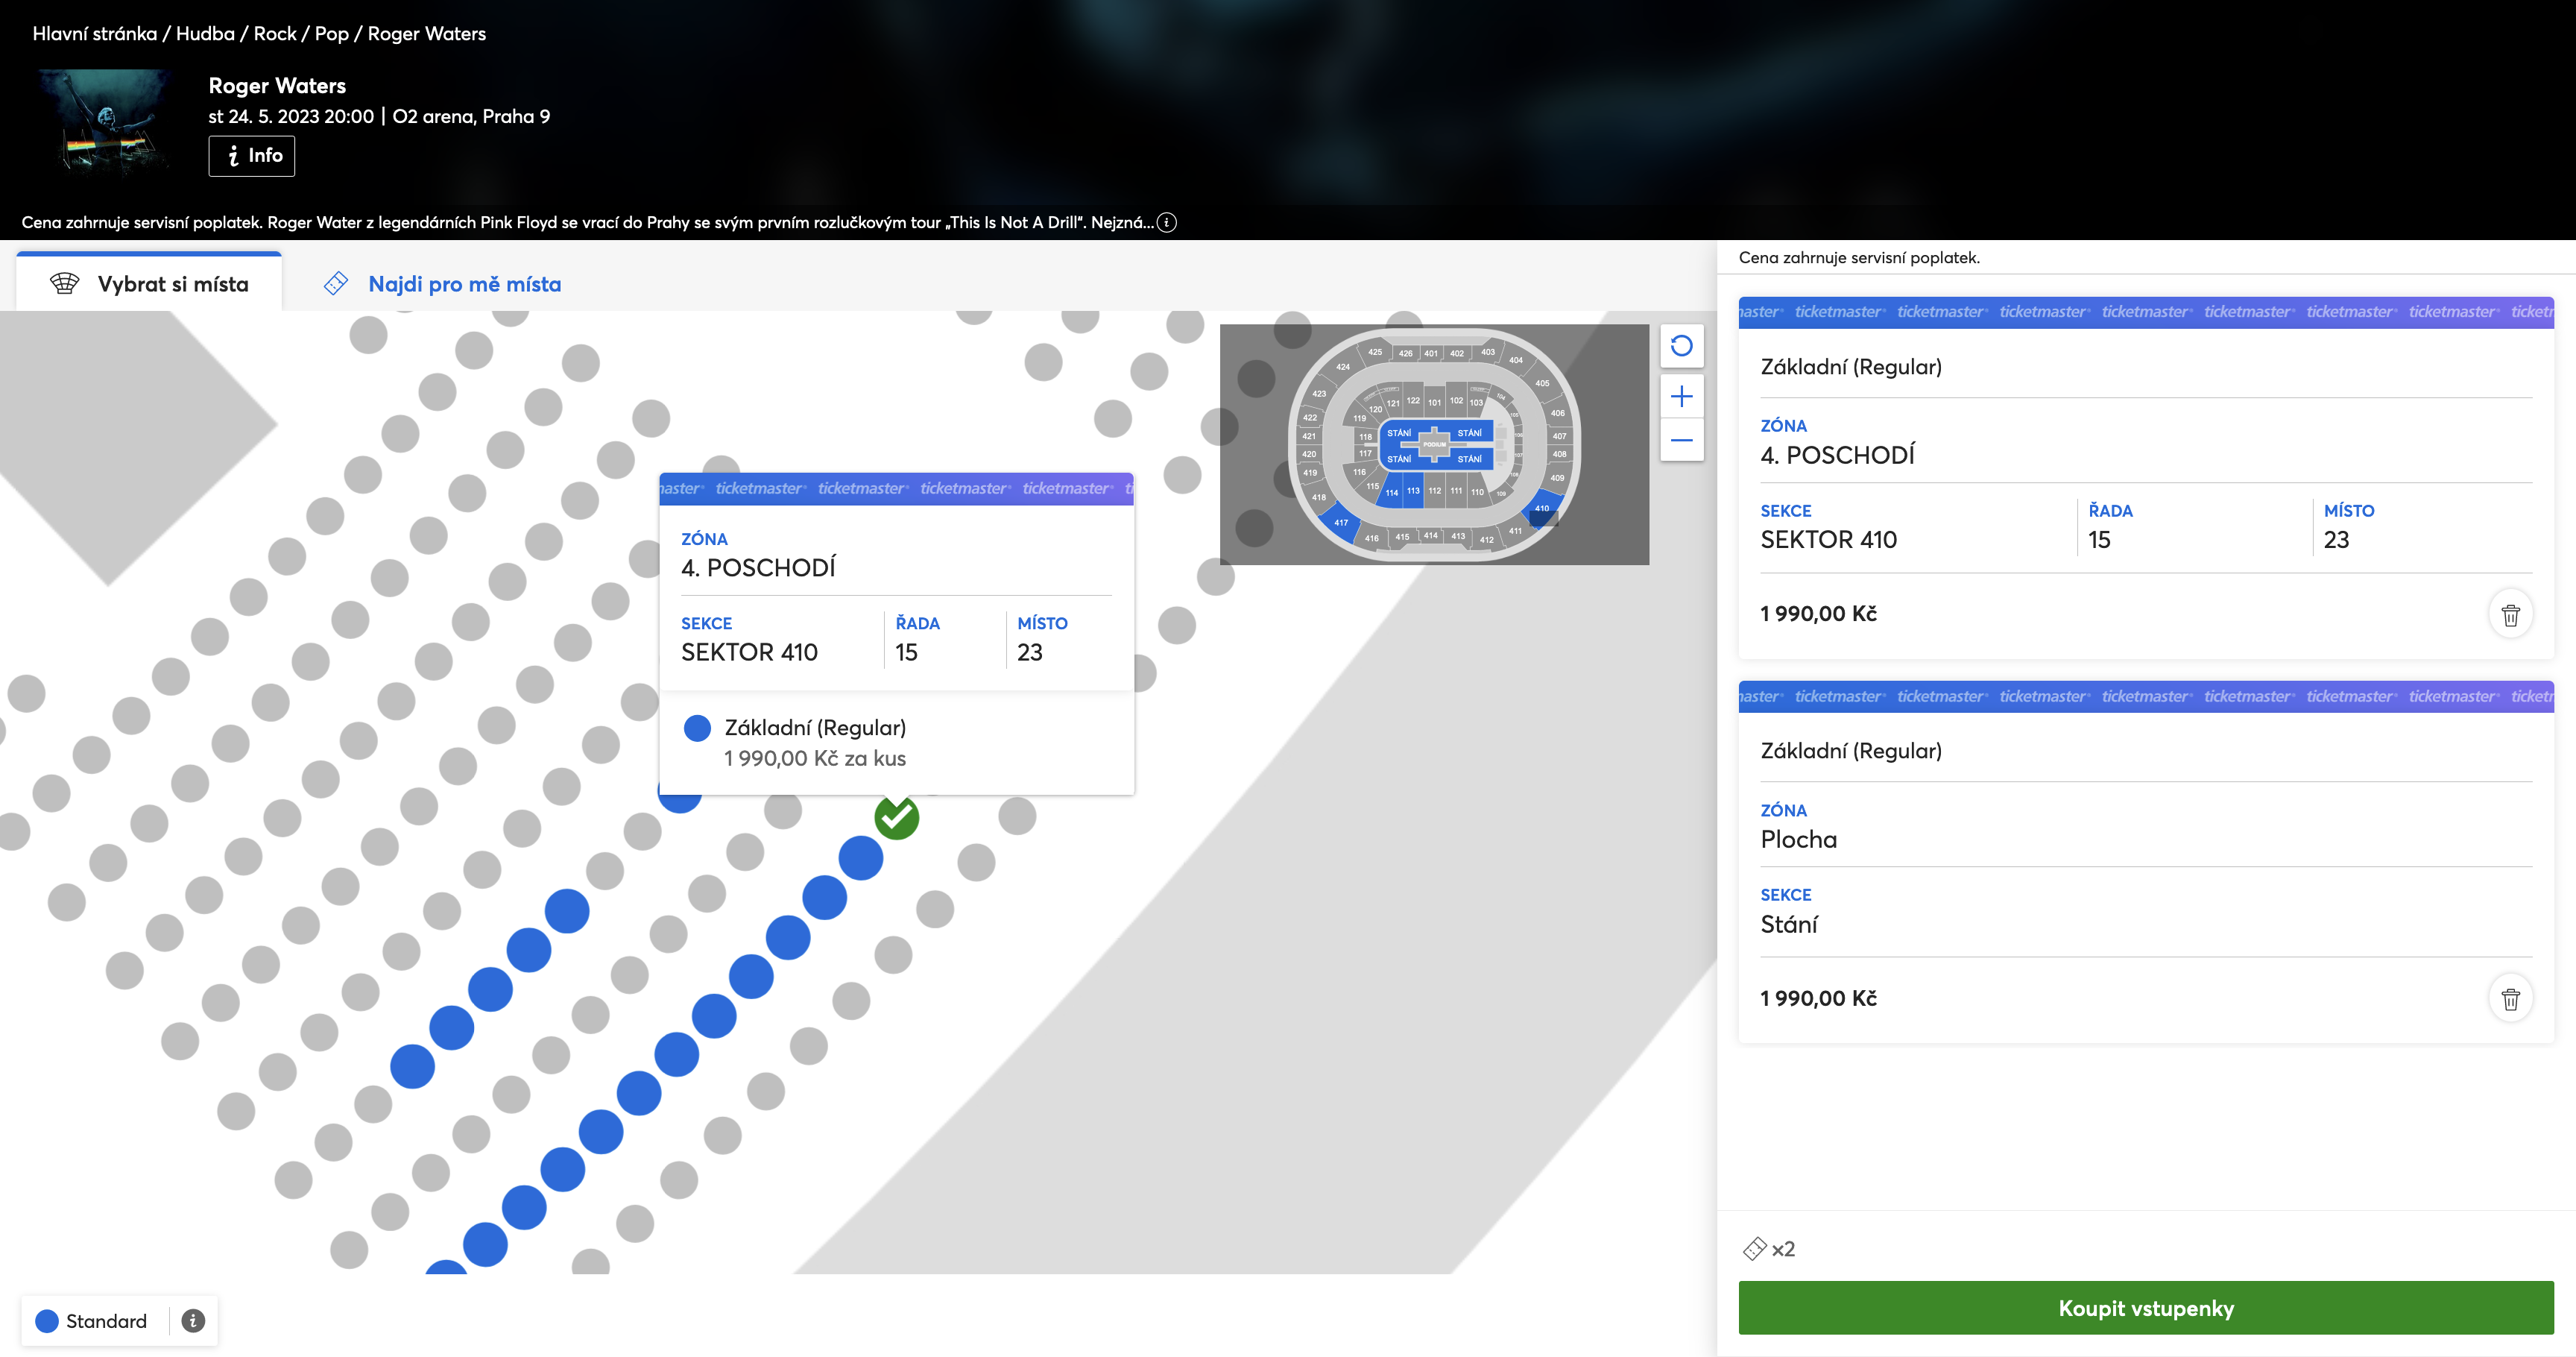
\includegraphics[width=\linewidth]{\FIGDIR/ticketmaster-cart-overview}
    \centering
    \caption{Nákupní košík na portálu Ticketmaster.com}
    \label{fig:ticketmaster-cart-overview}
\end{figure}

Nákupní košík by zároveň měl zobrazit přehled cen jednotlivých položek a celkovou cenu objednávky včetně všech daní a dalších případních poplatků.
Tato funkcionalita zákazníkovi zajišťuje naprostou transparentnost v nabízených službách a umožňuje mu předem zkontrolovat celkovou cenu objednávky.

\begin{figure}[H]
    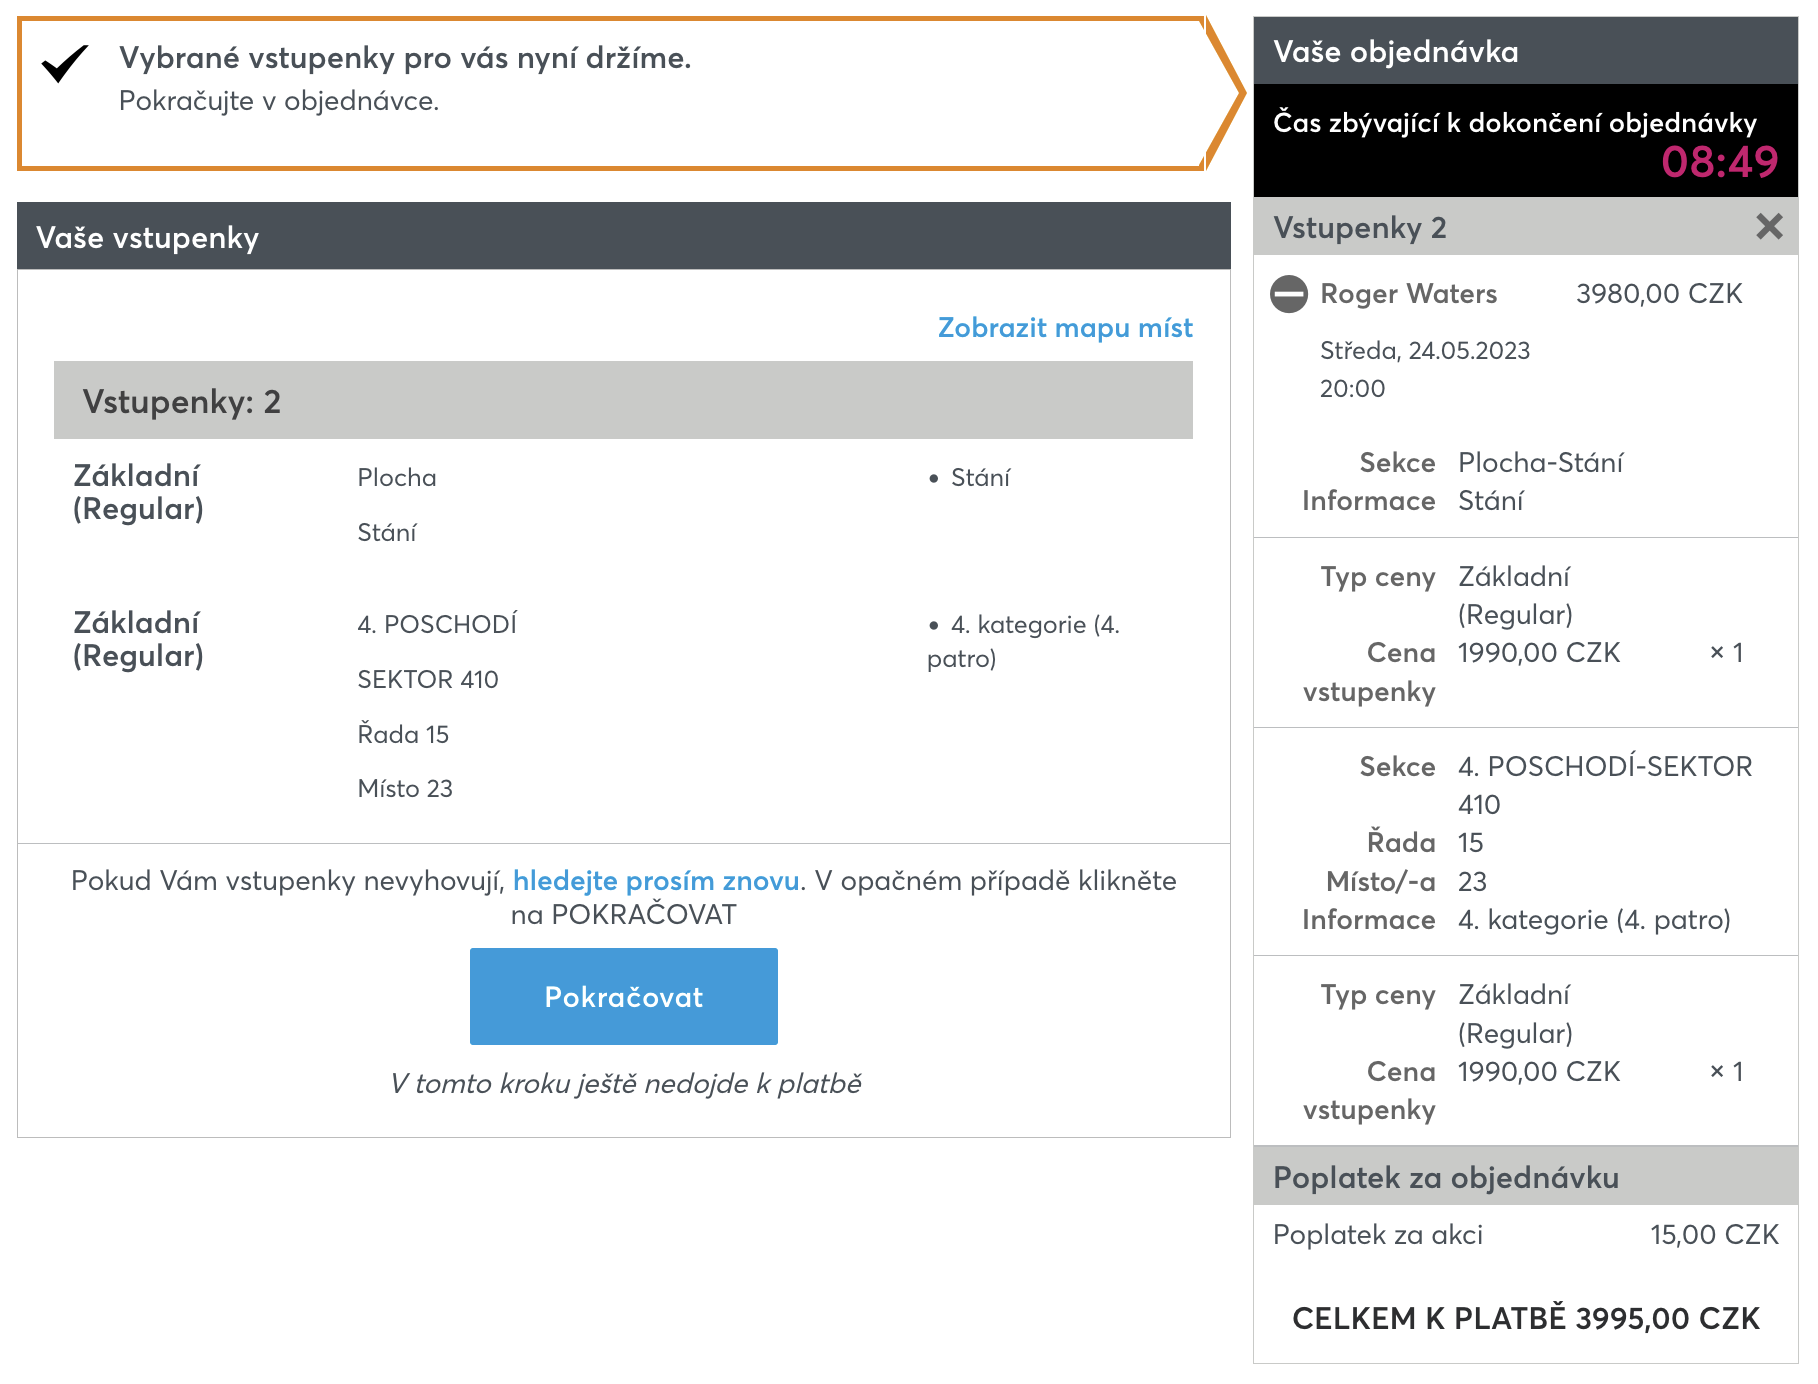
\includegraphics[width=\linewidth]{\FIGDIR/ticketmaster-cart-summary}
    \centering
    \caption{Souhrn objednávky na portálu Ticketmaster.com}
    \label{fig:ticketmaster-cart-summary}
\end{figure}


%%% Podsekce - Rezervace míst
%%%%% Wording: ⏳
%%%%% Styling: ⏳
%%%%% References: ⏳
%%% --------------------------------------------------------------
\subsection{Rezervace míst}
\label{subsec:specifikace-nakupni-kosik-rezervace}
V rámci nákupního procesu si zákazník vybírá místa, které jsou dostupná a při jejich výběru se zákaznikovi přidají do nákupního košíku.
Tato vybraná místa zákazníkem by se měla rezervovat, aby se předešlo nepříjemným situacím při dokončení objednávky, kdy zákazník zjistí, že jeho vybrané místo je již obsazené.

V případně aplikace, která se primárně zaměřuje na rezervací míst při prodeji vstupenek je tato funkcionalita naprosto esenciální.
Zákazník by měl mít možnost vybrat si místa, která jsou v danou chvíli dostupná a při jejich výběru by se měla pomocí rezervačnícho mechanismu v rámci vytvářené objednávky zákazníkovi zarezervovat a garantovat mu v případně dokonení objednávky jejich dostupnost.

Tento rezervační systém by měl dále implementovat funkčnost časového omezení rezervace, která zajistí uvolnění rezervovaných míst po uplynutí určitého časového limitu.
Tato funkčnost je velmi důležitá pro zajištění dostupnosti míst pro všechny zákazníky a zabraňuje zarezervování sedadel, která by nebyla zakoupena například z důvodu opuštění nákupního procesu zákazníkem.

V rámci tohoto rezervačního mechanismu by také mělo být zákazníkovi jasně zobrazeno, že má určitý časový limit, ve rámci kterého musí svou objednávku dokončit, jinak se jeho rezervace uvolní a bude si muset místa vybrat znovu.

\begin{figure}[H]
    \centering
    \begin{subfigure}{0.3\textwidth}
        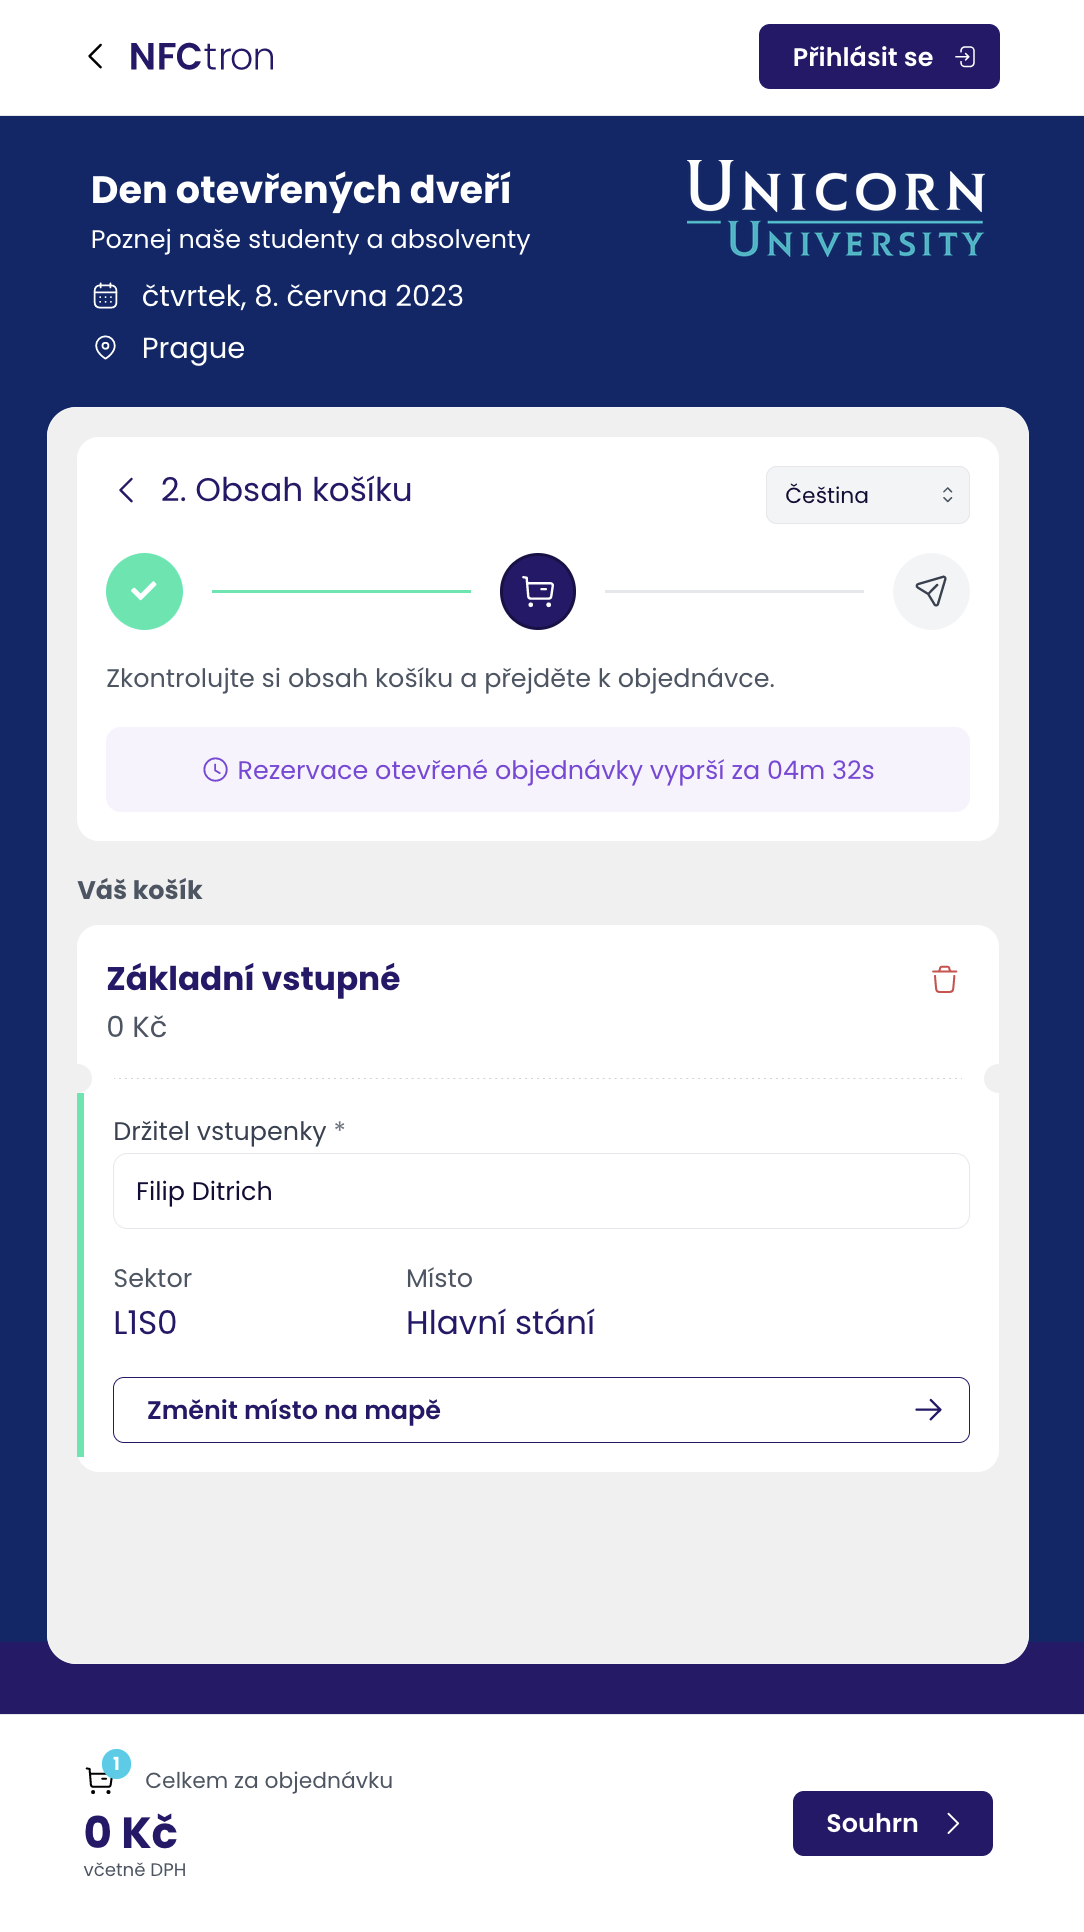
\includegraphics[width=\textwidth]{\FIGDIR/nfctron-tickets-reservation-pending}
        \caption{Běžící rezervace}
        \label{fig:nfctron-tickets-reservation-pending}
    \end{subfigure}
    \hfill
    \begin{subfigure}{0.3\textwidth}
        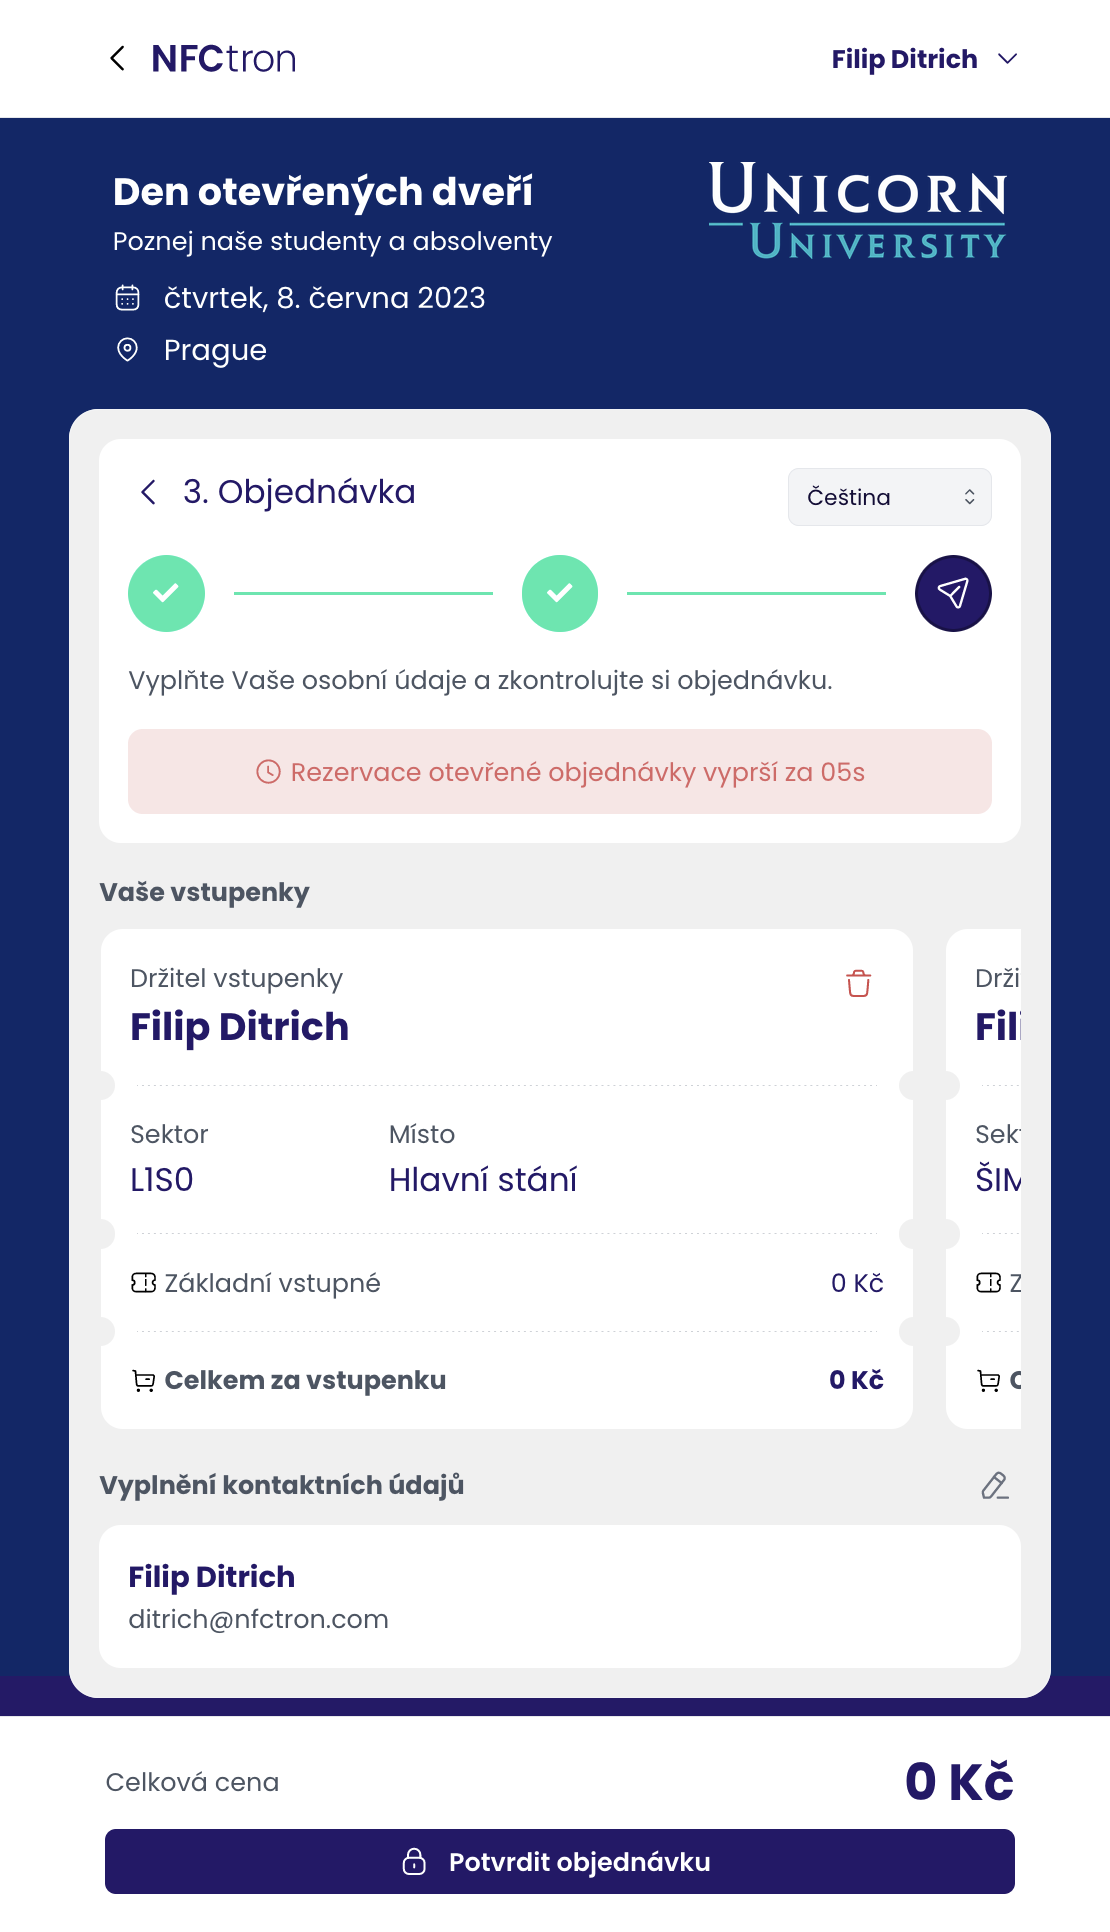
\includegraphics[width=\textwidth]{\FIGDIR/nfctron-tickets-reservation-expiring}
        \caption{Blížící se expirace}
        \label{fig:nfctron-tickets-reservation-expiring}
    \end{subfigure}
    \hfill
    \begin{subfigure}{0.3\textwidth}
        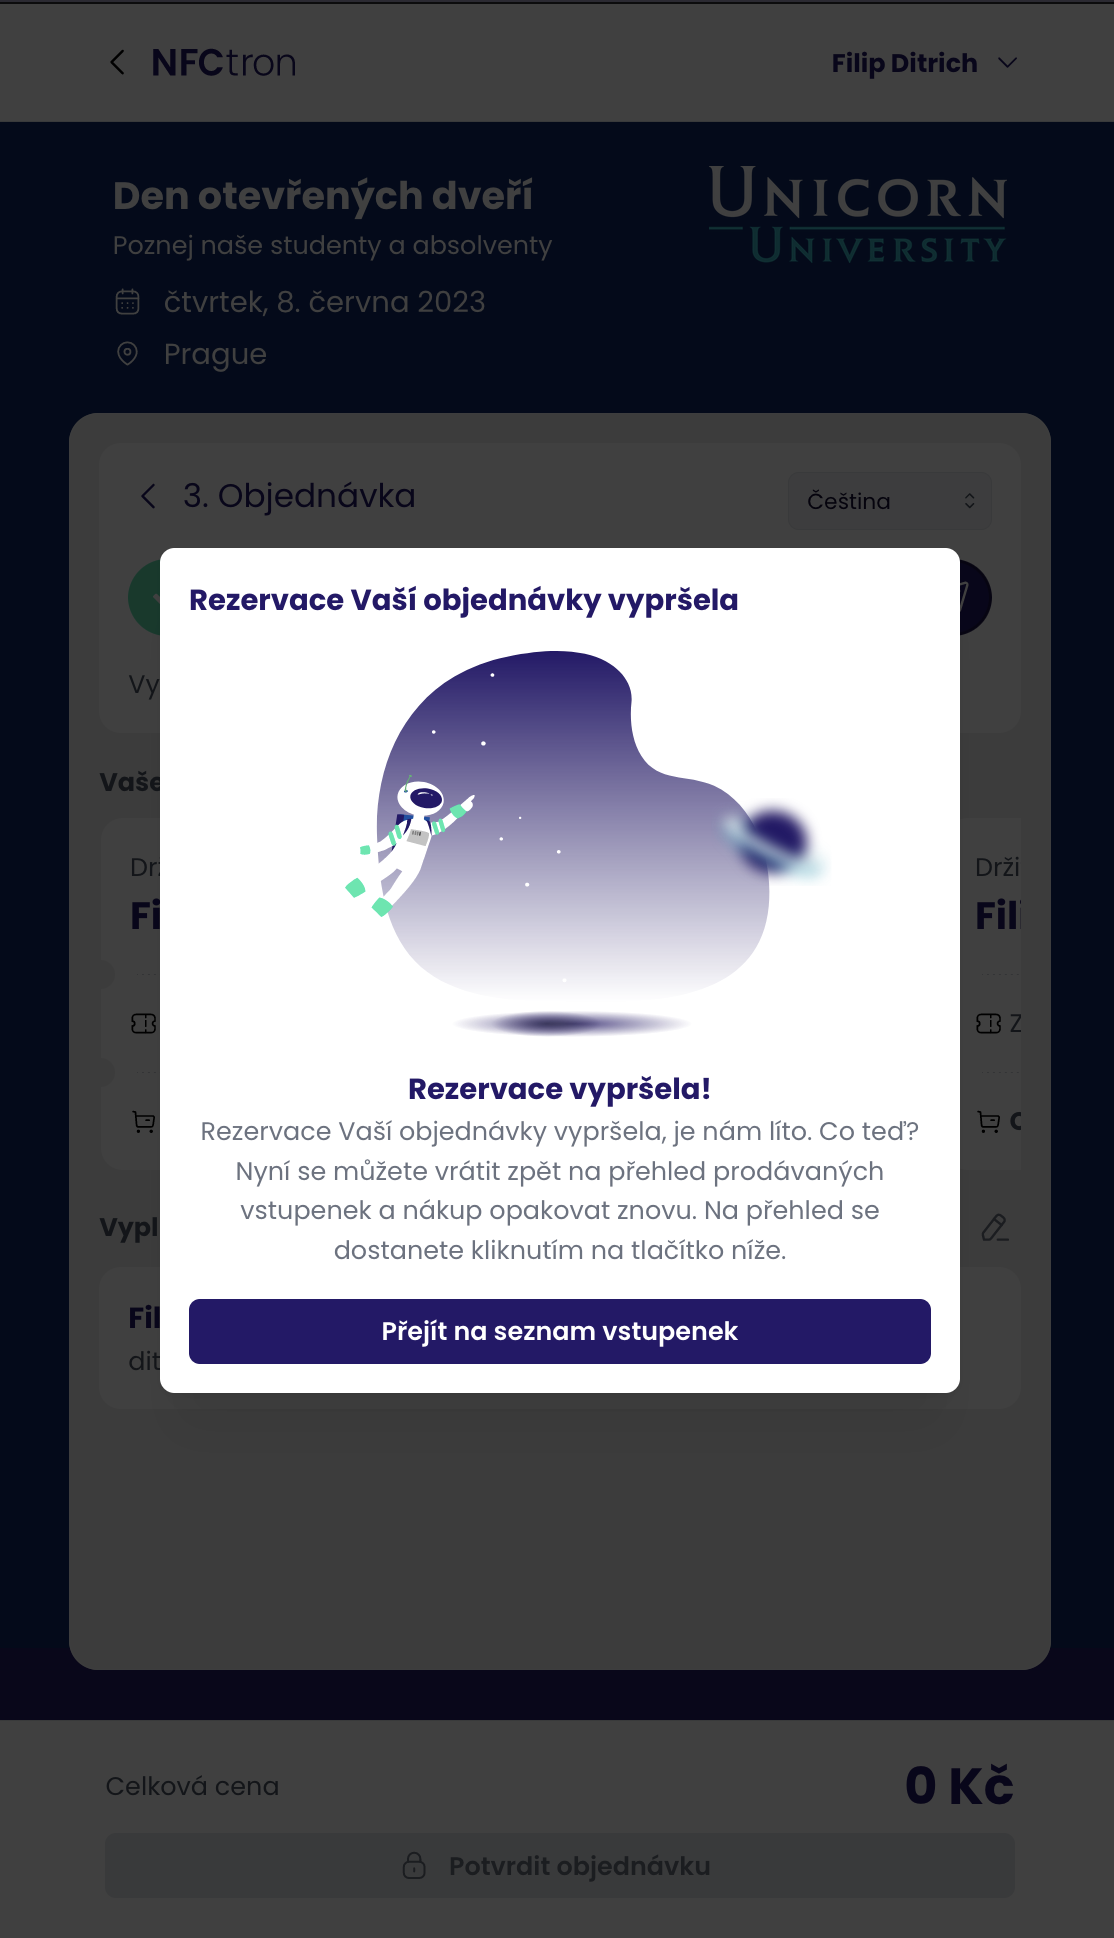
\includegraphics[width=\textwidth]{\FIGDIR/nfctron-tickets-reservation-expired}
        \caption{Expirovaná rezervace}
        \label{fig:nfctron-tickets-reservation-expired}
    \end{subfigure}

    \caption{Rezervační mechanismus služby NFCtron Tickets na zkušební akci}
    \label{fig:nfctron-tickets-reservation}
\end{figure}

%%% Sekce - Dokončení objednávky
%%%%% Wording: ⏳
%%%%% Styling: ⏳
%%%%% References: ⏳
%%% --------------------------------------------------------------
\section{Dokončení objednávky}
\label{sec:specifikace-dokonceni-objednavky}
Jakmile si zákazník vybere požadované vstupenky a rezervovaná místa, je jeho posledním úkolem dokončit a tím tak vytvořit objednávku, kteoru následně zaplatí.
Tento proces je většinou rozdělen do několika kroků, které zákazníka postupně provedou celým procesem dokončení objednávky.

Tato podkapitola se bude těmito kroky zabývat a bude se snažit popsat jejich jednotlivé části a funkčnosti, které by měly být v takovémto systému implementovány.

Avšak je nutné nejprve uvést, že následující funkčnosti jsou v práci uvedené pouze z důvodu kompletnosti představení celého procesu nákupu vstupenek s rezervací míst a záměrně nebudou v rámci praktické části plně implementovány nýbrž pouze orientačně využity – a to z důvodu toho, že se jedná již převážně o funkčnosti a procesy na straně backednového systému a ne frontendového, který je předmětem této práce.

%%% Podsekce - Osobní informace
%%%%% Wording: ⏳
%%%%% Styling: ⏳
%%%%% References: ⏳
%%% --------------------------------------------------------------
\subsection{Osobní informace}
\label{subsec:specifikace-dokonceni-objednavky-osobni-informace}
Pro účely dokončení objednávky je nutné, aby si zákazník vyplnil své osobní informace, které jsou potřebné pro vytvoření objednávky a následné doručení vstupenek.
Tyto informace by měly obsahovat minimálně následující údaje:

\begin{itemize}
    \item Jméno a příjmení
    \item Emailová adresa
    \item Telefonní číslo
\end{itemize}

Tyto informace jsou nezbytné například pro odeslání potvrzení objednávky, doručení vstupenek či poskytování případné podpory zákazníkům.

Někteří poskytovatelé stále nabízí doručení fyzických vstupenek na adresu zákazníka, nicméně tento způsob je spíše přežitek.
V dnešní moderní době je výhodnější i ekologičtější využít možnost digitálních vstupenek, které zákazník obdrží v elektronické podobě například prostřednictvím emailu či SMS zprávy.

V rámci dokončení objednávky je také časté vybídnutí zákazníka k dokončení registrace na dané platformě či službě, přes kterou vstupenky nakupuje.
Tato registrace je většinou dobrovolná, ale může být i povinná, pokud chce zákazník využít některé z výhod, které jsou s touto registrací spojeny.

%%% Podsekce - Výběr platební metody
%%%%% Wording: ⏳
%%%%% Styling: ⏳
%%%%% References: ⏳
%%% --------------------------------------------------------------
\subsection{Výběr platební metody}
\label{subsec:specifikace-dokonceni-objednavky-vyber-platebni-metody}
Proces dokončení objednávky by v posledním kroku měl zákazníkovi nabídnout několik možností platby.
Nejčastěji se jedná o platební metody jako:

\begin{itemize}
    \item platba kartou
    \item platba přes PayPal
    \item platba přes Apple Pay
    \item platba přes Google Pay
    \item platba přes bankovní převod
\end{itemize}

\begin{figure}[H]
    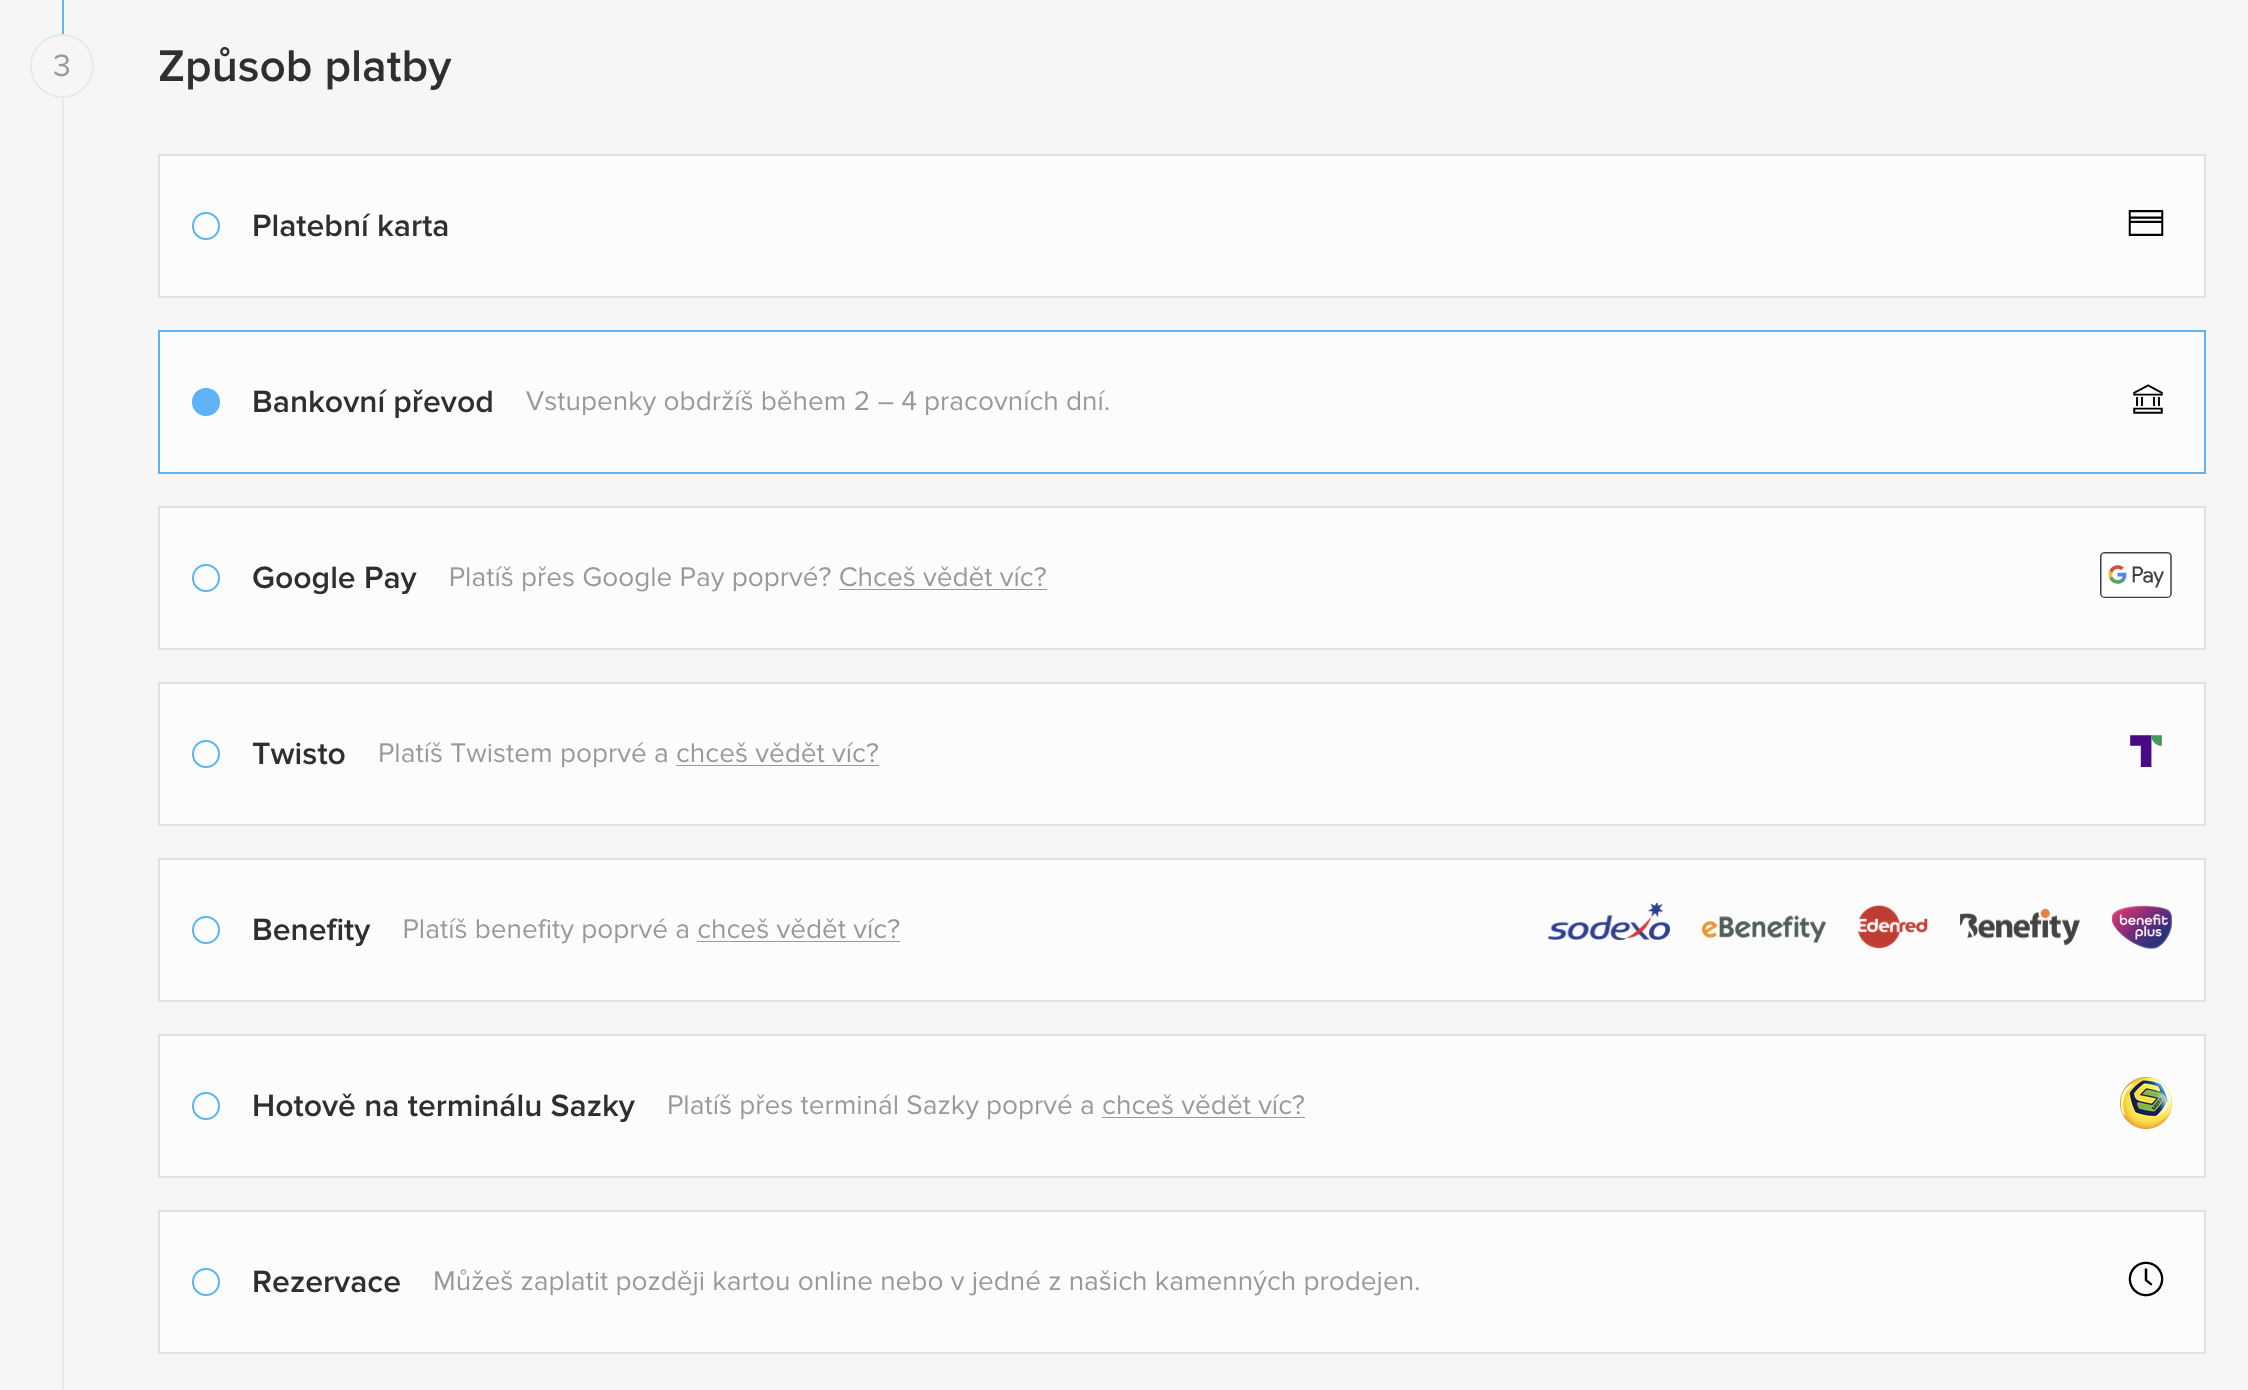
\includegraphics[width=\linewidth]{\FIGDIR/goout-payment-methods}
    \centering
    \caption{Vyběr platební metody na GoOut.net}
    \label{fig:goout-payment-methods}
\end{figure}

Na obrázku~\ref{fig:goout-payment-methods} je vidět výběr platební metody ve službě GoOut.net, která nabízí výše zmíněné platební metody\footnote{platební metoda Apple Pay zde není uvedena, jelikož je dostupná pouze v rámci prohlížečů Safari: \url{https://support.apple.com/guide/iphone/use-apple-pay-in-apps-app-clips-and-safari-iph67e89f7c8/ios}} spolu i dalšími jako například platba přes službu Twisto či Sodexo a další jiné benefitní programy.

Pro účely platby kartou je nutné, aby byl zákazník přesměrován na platební bránu, která je schopna tuto platbu zpracovat.
Většinou se jedná o platební brány třetích stran, které jsou schopny zpracovat platby z různých platebních karet a poskytovatelů.
Mezi nejznámější poskytovatele platebních brán na českém trhu patří například:

\begin{itemize}
    \item \emph{Comgate} (\url{https://www.comgate.cz/platebni-brana})
    \item \emph{GoPay} (\url{https://www.gopay.com/cs/})
    \item \emph{PayU} (\url{https://czech.payu.com/payu-moderni-platebni-reseni/})
    \item \emph{GP webpay} (\url{https://www.gpwebpay.cz/})
    \item \emph{Stripe} (\url{https://stripe.com/en-cz})
\end{itemize}

Na obrázcích~\ref{fig:comgate-fees-table} a~\ref{fig:comgate-payment-methods} je vidět, že každý poskytovatel platební brány nabízí jiné výhody a poplatkové modely, nicméně všechny mají společné to, že zpracovávají platby z různých platebních karet a poskytovatelů a přímo podporují i mobilní platby přes Apple Pay a Google Pay.

\begin{figure}[H]
    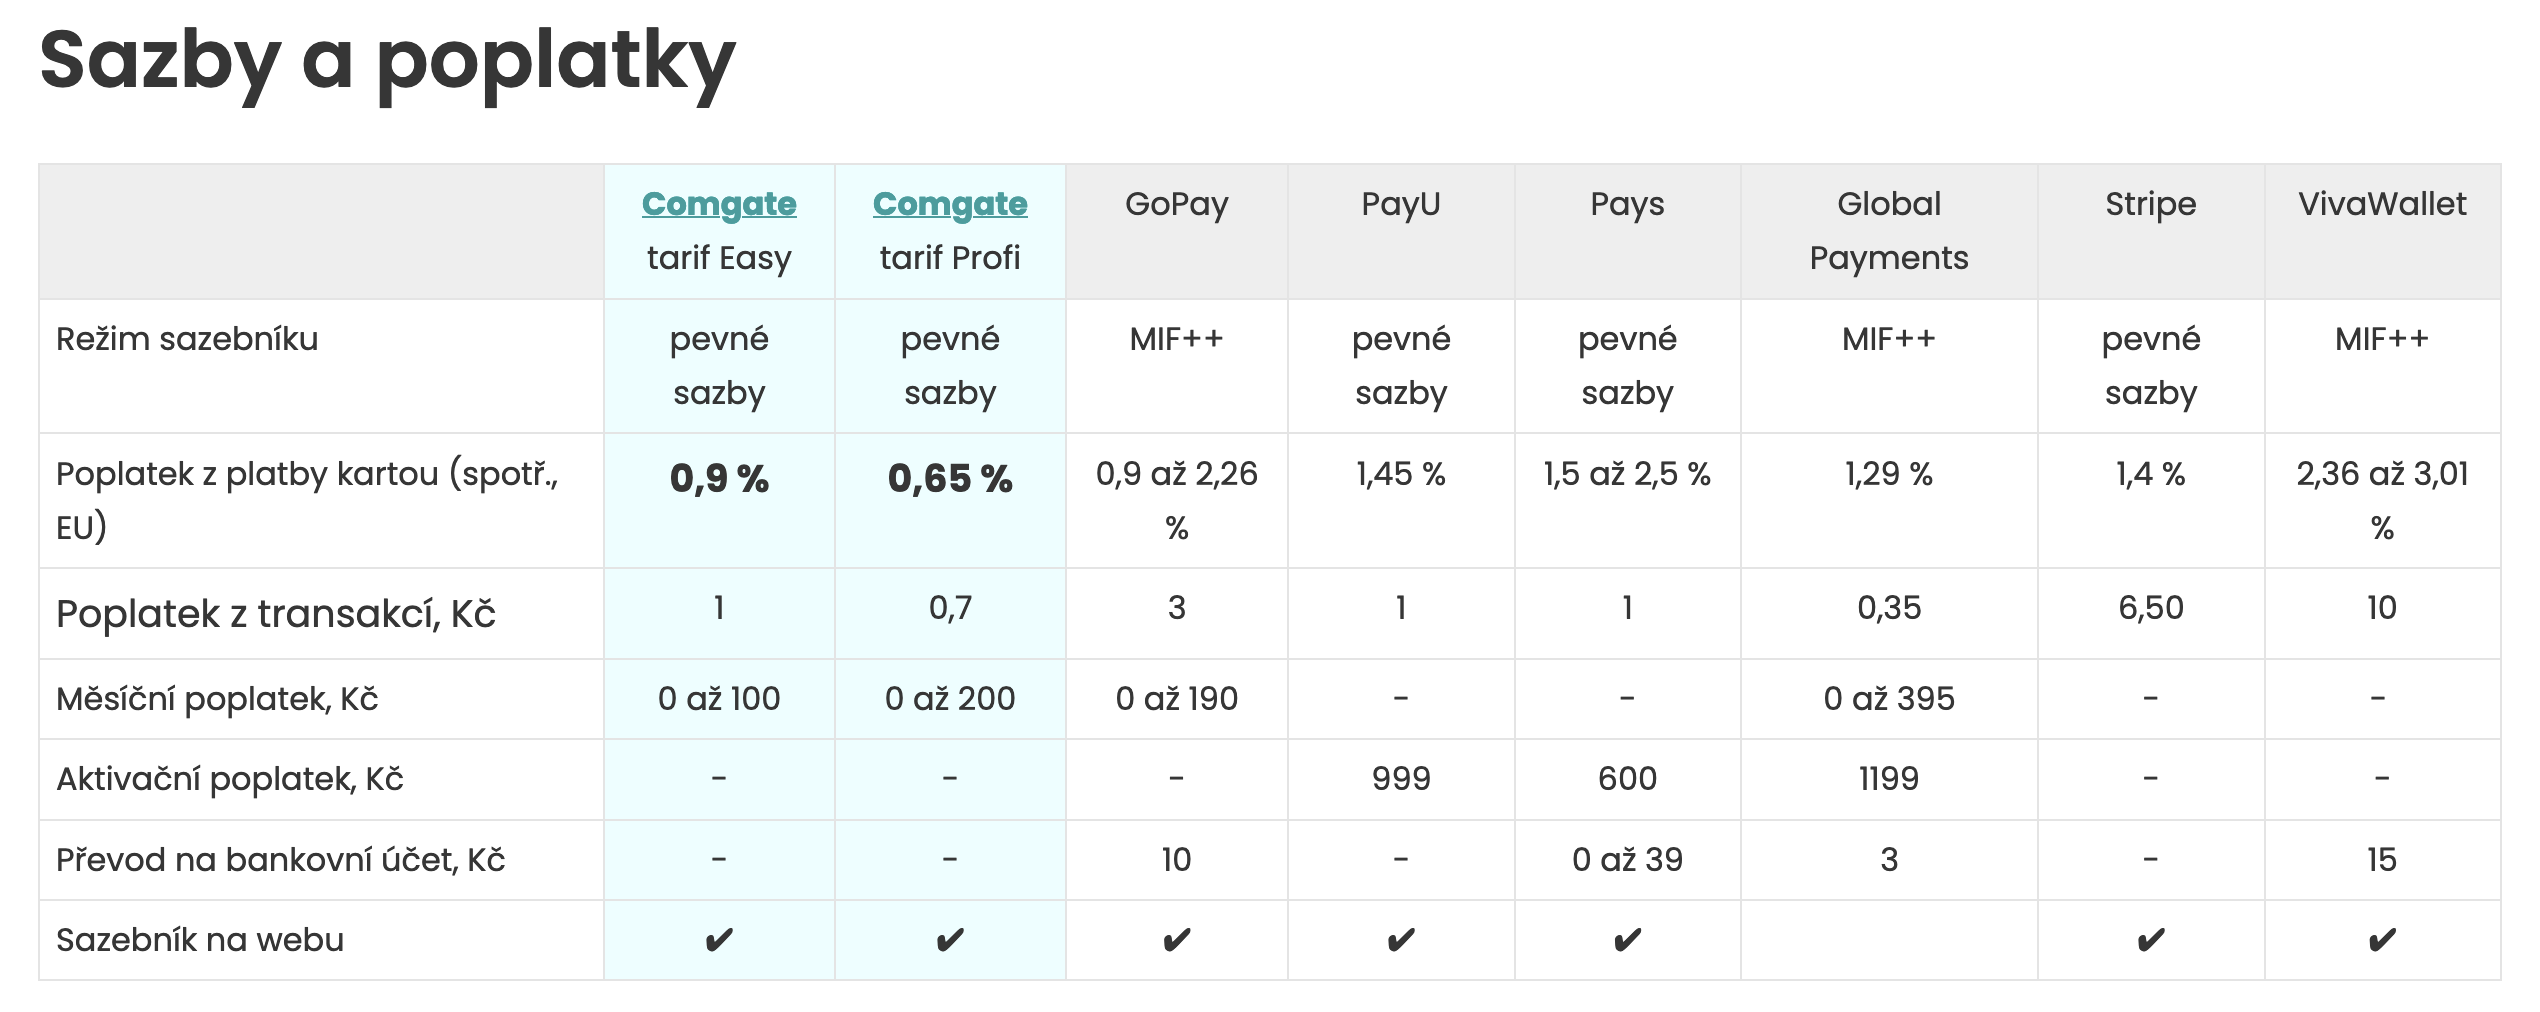
\includegraphics[width=\linewidth]{\FIGDIR/comgate-fees-table}
    \centering
    \caption{Srovnání platebních bran dle Comgate.cz~\cite{comgate_srovnani_platebnich_bran}}
    \label{fig:comgate-fees-table}
\end{figure}

\begin{figure}[H]
    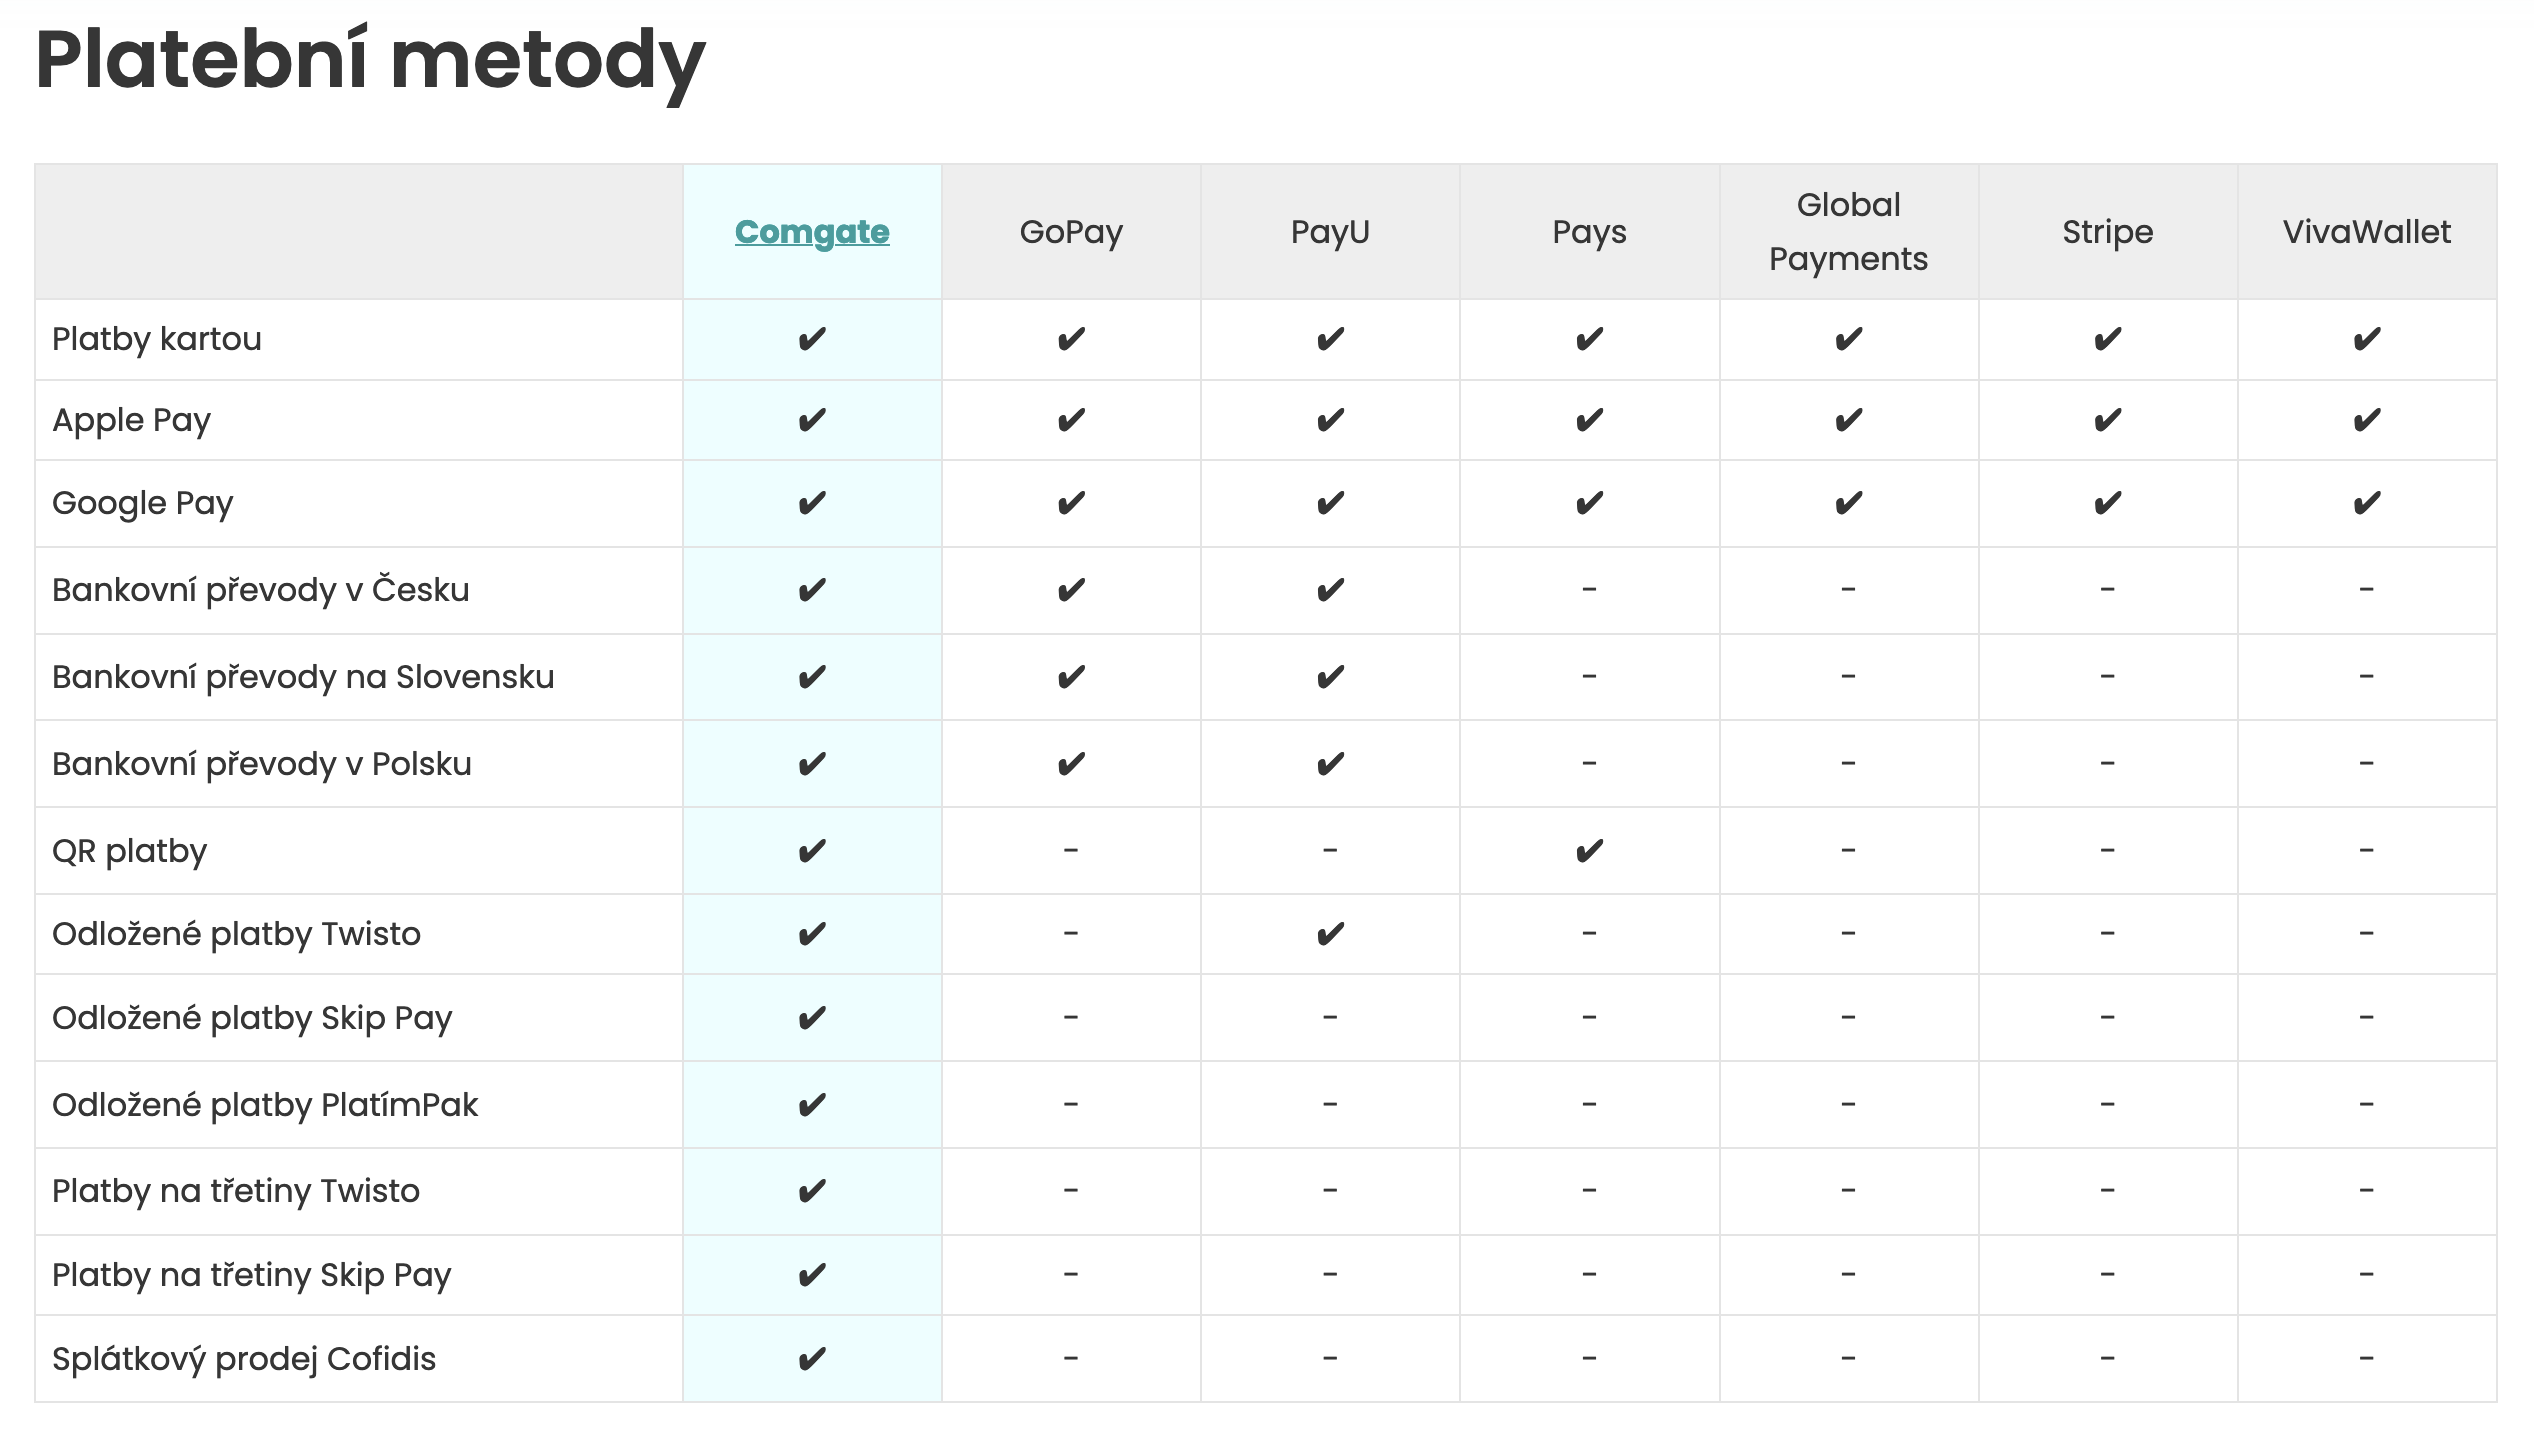
\includegraphics[width=\linewidth]{\FIGDIR/comgate-payment-methods}
    \centering
    \caption{Platební metody poskytované platebními poskytovateli dle Comgate.cz~\cite{comgate_srovnani_platebnich_bran}}
    \label{fig:comgate-payment-methods}
\end{figure}

Některé e-shopy však nabízí i vlastní platební bránu, nicméně tato možnost je spíše výjimkou.
Stát se provozovatelem vlastní platební brány je totiž velmi náročné na vývoj, udržbu a provoz a je k němu nutné mít i licenci platební instituce (PI)~\cite{schejbal_platebni_instituce}, kterou vydává Česká národní banka (ČNB)~\cite{cnb_dohled_platebni_instituce}.

Platby přes bankovní převod mohou být pro poskytovatele řešení prodeje vstupenek velmi výhodné, jelikož se jedná o levnější způsob převodu peněz, než je tomu u plateb kartou.
Platební brány si totiž účtují poplatky za zpracování každé z plateb a to nejčastěji v režimu pevného sazebníku či MIF++ modelu\footnote{někdy také označován jako Interchange++}, který rozděluje poplatky mezi vydavatelskou bankou, karetním schématem (např.\ Visa, MasterCard) a platební bránou.

Do nedávna byla platba bankovním převodem pro zákazníky stále méně oblíbená, jelikož bylo nutné počkat na připsání peněz na účet poskytovatele, což mohlu trvat i několik dní.
V dnešní době je však možné využít tzv.
instantní platby, které jsou schopny převést peníze mezi účty různých bank během několika sekund.
V České republice aktuálně podporuje instantní platby již několik bank, jako například Komerční banka, a.s., MONETA Money Bank, a.s.\ či Fio banka, a.s.\ a další\footnote{kompletní seznam účastníků okamžitých plateb dle ČNB dostupný z: \url{https://www.cnb.cz/export/sites/cnb/cs/platebni-styk/.galleries/certis/download/seznam_okamzite_platby.pdf}}.

Pro účely této práce, jak bylo již zmíněno na začátku podsekce~\ref{sec:specifikace-dokonceni-objednavky}, bude backendový systém celou funkčnost plateb pouze simulovat a nebude se snažit o integraci s žádnou platební bránou.


%%% Podsekce - Souhrn objednávky
%%%%% Wording: ⏳
%%%%% Styling: ⏳
%%%%% References: ⏳
%%% --------------------------------------------------------------
\subsection{Souhrn objednávky}
\label{subsec:specifikace-dokonceni-objednavky-souhrn-objednavky}
Po vyplnění všech potřebných informací a výběru platební metody by zákazníkovi měl být před finálním potvrzením objednávky zobrazen její souhrn.
Tento souhrn zákazníkovi umožní zkontrolovat, zda jsou všechny údaje správně vyplněné a zda je vše v pořádku.
Pokud zákazník zjistí, že je něco špatně, měl by mít možnost vrátit se zpět a údaje opravit.
Pokud je vše v pořádku, měl by mít možnost objednávku potvrdit a přejít k platebnímu procesu.

Součástí potrvzení objednávky také často bývá zaškrtnutí souhlasu se zpracováním osobních údajů a obchodních podmínek či i případně dalších informací, jako například zasílání novinek a reklamních nabídek na e-mailovou adresu zákazníka.

%%% Podsekce - Vytvoření objednávky a potvrzení
%%%%% Wording: ⏳
%%%%% Styling: ⏳
%%%%% References: ⏳
%%% --------------------------------------------------------------
\subsection{Vytvoření objednávky a potvrzení}
\label{subsec:specifikace-dokonceni-objednavky-vytvoreni-objednavky-a-potvrzeni}
Po potvrzení objednávky by měla být vytvořena objednávka v databázi a zákazníkovi by mělo být zobrazeno potvrzení o jejím vytvoření.
Na základě vybrané platbní metody by měl být dále přesměrován k jejímu zaplacení a posléze zpět na detail objednávky s potrvzením o zaplacení.
Při úspěšné platbě by zákazníkovi měl systém doručit zakoupené vstupenky v elektronické podobě, například v podobě PDF souboru, který bude obsahovat vstupenky ve formátu QR kódu.
